\documentclass{article}
% PACKAGES
\usepackage[english]{babel}
\usepackage{graphicx} % Required for inserting images
\usepackage{lmodern}
\usepackage{tcolorbox}
\usepackage{amsmath}
\usepackage{pgfplots}
\usepackage{xcolor}
\usepackage{tikz}
\usepackage{color,soul}
\usepackage{enumerate}
\usepackage{enumitem}
\usepackage{cancel}
\usepackage{hyperref} 
\usepackage{tikzsymbols}
\usepackage{fontawesome5}
\usepackage[export]{adjustbox}
\usepackage{amssymb}
\usepackage{setspace}
\usepackage{sectsty}


\definecolor{antiquefuchsia}{rgb}{0.57, 0.36, 0.51}
\definecolor{carnationpink}{rgb}{1.0, 0.65, 0.79}
\definecolor{lavenderpurple}{rgb}{0.59, 0.48, 0.71}
\usetikzlibrary{positioning}



% COLOURS
\definecolor{Orchid}{RGB}{218, 112, 214}
\definecolor{snow}{rgb}{1.0, 0.98, 0.98}
\definecolor{mordantred19}{rgb}{0.68, 0.05, 0.0}
\definecolor{mistyrose}{rgb}{1.0, 0.89, 0.88}
\definecolor{nadeshikopink}{rgb}{0.96, 0.68, 0.78}
\definecolor{cadmiumgreen}{rgb}{0.0, 0.42, 0.24}
\definecolor{OliveGreen}{RGB}{85, 107, 47}
\definecolor{RoyalPurple}{RGB}{120, 81, 169}
\definecolor{NavyBlue}{RGB}{0, 0, 128}
\definecolor{CornflowerBlue}{RGB}{100, 149, 237}
\definecolor{Cerulean}{RGB}{0, 123, 167}
\definecolor{DarkOrchid}{RGB}{153, 50, 204}

\usetikzlibrary{positioning}
\usetikzlibrary{calc,arrows.meta}


\title{MCV4U - Calculus and Vectors}
\author{Made By Kensukeken}
\date{30 January 2024}

\begin{document}
\begin{titlepage}
    \centering
    
\begin{tikzpicture}[overlay, remember picture]
        % Background gradient
        \fill[black] (current page.south west) rectangle (current page.north east);
        \fill[left color=violet!80!black, right color=black!40!black] (current page.south west) rectangle (current page.north east);
        % Title
        \node[font=\sffamily\bfseries\Huge, text=white] (title) at (current page.center) {MCV4U - Calculus and Vectors};
        % Author
        \node[below=1cm of title, font=\sffamily\LARGE, text=white] {By Kensukeken};
        % Mathematical symbols and equations
        \node[below=2cm of title, font=\sffamily\Large, text=white] (equation) {$\int_a^b f(x) d x=\lim _{\substack{n \rightarrow \infty \\ \max \Delta x_i \rightarrow 0}} \sum_{i=1}^n f\left(\xi_i\right) \Delta x_i$};
        \node[below=1cm of equation, font=\sffamily\large, text=white] {ISBN: 123-456-789};
        % Colored rectangle
        \fill[lavenderpurple] (title.east) ++(2cm,0) rectangle ++(5cm,-7cm);
    \end{tikzpicture}
\end{titlepage}

\clearpage % New page

\thispagestyle{empty} % No page number

\begin{center}
    
\includegraphics[width=0.5\textwidth]{imgs/OIG4.png} % Adjust the width as needed
\end{center}

\vspace{2cm}

\begin{center}
    \Huge\textbf{Calculus and Vectors}
\end{center}

\vspace{2cm}



\maketitle

\tableofcontents
\newpage



\subsection{Introduction}
\textbf{What is Calculus?}\\
Two simple geometric problems originally led to the development of what is now called calculus. Both problems can be stated in terms of the graph of a function $y=f(x)$.
\begin{itemize}
    \item The problem of tangents: What is the slope of the tangent to the graph of a function at a given point P?
    \item The problem of areas: What is the area under a graph of a function $y=f(x)$ between $x=a$ and $x=b$.
\end{itemize}
    \begin{figure}[ht]
    \centering
    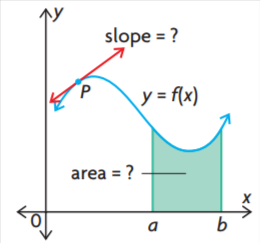
\includegraphics[width=0.35\textwidth]{imgs/Chapter 1 - MCV4U Nelson.png}
    \end{figure}
Isaac Barrow, a professor at the University of Cambridge, recognized the connection between the problem of tangents and the problem of areas. Newton and Gottfried Wilhelm von Leibniz independently solved these problems using differentiation and integration, a major advance in mathematics. This discovery led to the creation of calculus, a powerful branch of mathematics used in applied mathematics, science, engineering, and economics. The study of calculus begins with the meaning of a tangent, rate of change, limits, and the derivative of a function.
\newpage

\subsection*{Radical Expressions: Rationalizing Denominators}
In calculus, rationalizing the denominator of radical expressions involves simplifying expressions with radicals in the denominator. This process simplifies numbers into integers, making dividing by an integer more preferable than dividing by a radical number. \\ 

\subsection*{\textcolor{blue}{Selecting a strategy to rationalize the denominator}}
\begin{align*}
&\text{Simplify the radical expression } \frac{5}{2 \sqrt{6}+3} \text{ by rationalizing the denominator.} \\
&\text{Solution} \\
&\frac{5}{2 \sqrt{6}+3} = \frac{5}{2 \sqrt{6}+3} \times \frac{2 \sqrt{6}-3}{2 \sqrt{6}-3} \quad \text{(The conjugate $2 \sqrt{6}+\sqrt{3}$ is $2 \sqrt{6}-\sqrt{3}$)} \\
&= \frac{5(2 \sqrt{6}-3)}{4 \sqrt{36}-9} \\
&= \frac{5(2 \sqrt{6}-3)}{24-9} \\
&= \frac{5(2 \sqrt{6}-3)}{15} \\
&\text{(Divide by the common factor of 5)} \\
&= \frac{2 \sqrt{6}-3}{3}
\end{align*}
\\\\
When the denominator of a radical fraction is a two-term expression, you can rationalize the denominator by multiplying by the \textbf{\textcolor{blue}{conjugate}}. \\ \\
An expression such as $\sqrt{a}+\sqrt{b}$ has $\sqrt{a}-\sqrt{b}$ the conjugate.\\\\
Why are conjugates important? Recall that the linear terms are eliminated when
expanding a difference of squares. For example,
\begin{align*}
    (a-b)(a+b)&=a^2+ab-ab-b^2 \\
    &=a^2-b^2
\end{align*}
If a and b were radicals, squaring them would rationalize them.
\begin{align*}
\text{Consider this product:}\quad
    &(\sqrt{x}-\sqrt{y})(\sqrt{x}+\sqrt{y}), \; x, \text{y rational} \\ &=(\sqrt{x})^2+\sqrt{xy}-\sqrt{xy}-(\sqrt{x})^2 \\
    &=x-y \quad \textbf{Notice that the result is rational!}
\end{align*}

\newpage
\section{Unit 1 - Limits}
\subsection{Evaluating Limits Graphically}
Imagine someone is standing 10 metres from a wall. We tell that person to move halfway to the wall. We then them to again move halfway to the wall. We then tell them to again move halfway to the wall, and we continue to do this. Theoretically, the person will never reach the wall. However, we can say that as the number of trials moves to infinity, the limit of where the person is standing will be the wall.

Of course, the person will never each the wall(theoretically), but we could still refer to the wall as the limit.

Another way to think about limits is to think about sequnces.

Consider the sequence $f(n)$ where n is a positive integer referring to the ordinal position of the term in the sequence and $f(n)$ is the value of that term.
$$1,\frac{1}{2},\frac{1}{4},\frac{1}{8},\frac{1}{16}, \cdots $$
The values are getting closer and closer to 0. We know that the values will never reach 0, but they will get infinitely close to 0. We can say that the limit of the sequence as the number of terms goes to infinity is 0.

$$\lim_{n \to \infty} f(n)=0$$
In mathematics, a limit is the value that a function(or sequence) "approaches" as the input (or index) "approaches" some value. Limits are essential to calculus(and mathematical analysis in general) and are used to define continuity, derivatives, and integrals.When dealing with functions, we can let the x-value inputted to the function grow closer and closer to some set value. We then watch the pattern of y-values to see if there is a set y-value that we grow infinitely close to. If there is such a value, we say that that is the value of the limit

\subsubsection{Example:}
Suppose that we wish to determine $\lim_{x \to 3} (-x^2+6x-5 )$. We can draw the graph of $y=-x^2+6x-5$:

\begin{minipage}{0.6\textwidth}
    \begin{align*}
        \lim_{x \to 3^-} f(x) &= 4 \\
        \lim_{x \to 3^+} f(x) &= 4 \\
        \lim_{x \to 3} f(x) &= 4
    \end{align*}
\end{minipage}%
\vspace{0.1em}%
\begin{minipage}{0.6\textwidth}
    The graph of $y=-x^2+6x-5$:
    \begin{center}
        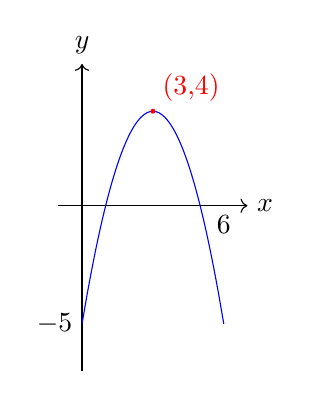
\begin{tikzpicture}[scale=0.3]
            % Axis
            \draw[->] (-1,0) -- (7,0) node[right] {$x$};
            \draw[->] (0,-7) -- (0,6) node[above] {$y$};
          
            % Function plot
            \draw[domain=0:6, smooth, variable=\x, blue] plot ({\x}, {-\x^2 + 6*\x - 5});
            \fill[red] (3, 4) circle (3pt) node[above right] {(3,4)};

          
            % Labels
            \node[below] at (6,0) {$6$};
            \node[left] at (0,-5) {$-5$};
        \end{tikzpicture}
    \end{center}
\end{minipage}
When determining whether the limit as x approaches a particular value of a function exists, we compare the two one-sided limits and see if they are the same. If they are, then the limit exists, and is equal to that common value.
\\ 
\begin{tcolorbox}[colback=Orchid!5!white,colframe=cadmiumgreen!75!white,coltitle=white,]
If $\lim _{x \rightarrow a^{-}} f(x)=b$ and if $\lim _{x \rightarrow a^{+}} f(x)=b$ then $\lim _{x \rightarrow a} f(x)=b$
However, if $\lim _{x \rightarrow a^{-}} f(x)$ exists and if $\lim _{x \rightarrow a^{+}} f(x)$ exists but $\lim _{x \rightarrow a^{-}} f(x) \neq \lim _{x \rightarrow a^{+}} f(x)$, then $\lim _{x \rightarrow a} f(x)$ does not exist. \\ \\ 
\end{tcolorbox}

Note that in the last example, we expressed that limits were described as being equal to $\infty$ and to $-\infty$. Technically, nothing can be equal to $\infty$ or $-\infty$, so one could immediately conclude that $\lim_{x \to 4}\left( \frac{x+1}{x-4}\right)$ does not exist, as soon as one of the one-sided limits is equal to $\infty$ or $-\infty$. However, in this course, we will allow one-sided limits to be expressed as $\infty$ or $-\infty$. This will include limits as $x$ approaches $\infty$ or $-\infty$, which can only be approached from one direction. 

However, if we are seeking the limit of a function as $x$ approaches a real number (a two-sided limit), and if one of the one-sided limits is equal to $\infty$ or $-\infty$, then we will state that the limit of the function as $x$ approaches the real number does not exist.
\\
\subsubsection*{Limits that can only be approached from one side:}
Sometimes, we will come across a limit that can only be approached from the left or from the right. The most common type of limit of this form is when we seek to find the limit of a function as $x$ approaches $\infty$ or as $x$ approaches $-\infty$.

If we want to evaluate the limit of a function as $x$ approaches $-\infty$, we can only approach it from the right because we can’t be to the left of $-\infty$. Similarly, if we want to evaluate the limit of a function as $x$ approaches $\infty$, we can only approach it from the left because we can’t be to the right of $\infty$.

\begin{table}[h]
    \centering
    \begin{tabular}{|c|l|}
    \hline
    Expression & Explanation \\
    \hline
    $\frac{0}{0}$ & Indeterminate: maybe the limit and maybe it doesn't. Do more work! \\
    \hline
    $\frac{\text{Non-Zero}}{0}$ & The limit does not exist. You're done working. \\
    \hline 
    $\frac{\text{Anything}}{\text{Non-Zero}}$ & That's the answer :) \\
    \hline
    \end{tabular}
    \caption{Limit Evaluation Cases}
    \label{tab:limits}
\end{table}

\newpage

\subsection{Evaluating Limits Algebraically}
Assume that we are trying to evaluate $\lim_{x \to c}f(x), c \in \mathrm{R}$\\

We often don't use a graphing approach to evaluate a limit. Rather, we can use an algebraic approach if we remember the following steps. \\
\begin{enumerate}
    \item  \text{\hl{If the curve is continuous at $\mathrm{x}=\mathrm{c}$}}, then we can simply evaluate $\mathrm{f}(\mathrm{c})$. In other words, $\lim _{x \rightarrow c} f(x)=f(c)$ \\
    \begin{itemize}
        \item This happened in the first example in the powerpoint about evaluating limits graphically. When we were seeking to evaluate $\lim _{x \rightarrow 3}\left(-x^2+6 x-5\right)$, we could have recognized that this was a continuous function at $x=3$ and simply plugged in an $x$-value of 3 .
   \end{itemize}
\item \hl{However, sometimes direct substitution leads to a result of $0 / 0$.} Obviously, this result is undefined. However, the limit may still exist because there may be a hole at $\mathrm{x}=\mathrm{c}$ in an otherwise continuous curve.
\begin{itemize}
    \item This is what happened in some of our examples in the powerpoint on graphically evaluating limits. For example, in the example where we sought $\lim _{x \rightarrow-2}\left(\frac{x^2+3 x+2}{x+2}\right)$, there was a hole and the value of the limit equaled the $y$-coordinate of the location of the hole.
\end{itemize} 
When we get the indeterminate form of $0 / 0$, we can try the following:
\begin{tcolorbox}[colback=Orchid!5!white,colframe=Orchid!75!white,coltitle=white,]
\begin{enumerate}[label=(\roman*)]
    \item Factor numerator and denominator, and the offending factor may cancel out of both
    \item Rationalize the numerator and/or denominator and see if this leads you to be able to directly substitute
    \item Simplify the function prior to substituting to see if that allows you to directly substitute iv. Introduce a new factor that allows the numerator and/or denominator to become a difference or sum of nth powers, which then creates the offending factor which can then be canceled from both numerator and denominator (you may wish to introduce a new variable to do this)
\end{enumerate}
\end{tcolorbox}
\end{enumerate}
\newpage

\subsubsection{Examples where direct substitution leads to the correct answer}
\textbf{Examples}\\
1. Evaluate $\lim_{x \to 5}x^2+2x-3$
\begin{align*}
\lim_{x \to 5}x^2+2x-3 &= \text{Plug } x=5 \\ 
    &= (5)^2+2(5)-3 \\
    &= \boxed{32} \quad \text{That's the answer } 
\end{align*}
2. Evaluate $\lim_{x \to 3}\frac{\sqrt{x-1}-\sqrt{x+1}}{\sqrt{x-3}-\sqrt{x+3}}$\\
\begin{align*}
    &=\frac{\sqrt{3-1}-\sqrt{3+1}}{\sqrt{3-3}-\sqrt{3+3}}\\
    &=\frac{\sqrt{2}-\sqrt{4}}{\sqrt{0}-\sqrt{6}}\\
    &=\frac{\sqrt{2}-2}{-\sqrt{6}}
\end{align*}

2a)  Examples where Direct Substitution Leads to 0/0 But you can then factor, cross out, and then sub in\\\\
3. Evaluate $\lim_{h \to 0}\frac{(2+h)^3-8}{h}$
\begin{align*}
    &\text{Recall}: a^3-b^3 = (a-b)(a^2+ab+b^2)\\
    &=\lim_{h\to 0}\frac{\cancel{8}+12h^+6h^2+h^2\cancel{-8}}{h}\\
    &=\lim_{h\to 0}\frac{h^3+6h^2+12}{h}\\
    &=\lim_{h \to 0}\frac{\cancel{h}(h^2+6h+12)}{\cancel{h}}\\
    &= (0)^2+6(0)+12\\
    &=12
\end{align*}
4. Evaluate $\lim_{x \to 25}\frac{x-25}{\sqrt{x}-5}$
\begin{align*}
    &=\lim_{x \to 25}\frac{x-25}{\sqrt{x}-5} \times \frac{(\sqrt{x})^2-(5)^2}{\sqrt{x}-5}\\
    &=\lim_{x \to 25}\frac{\cancel{(\sqrt{x}-5)}(\sqrt{x}+5)}{\cancel{(\sqrt{x}-5)}}\\
    &=\sqrt{25}+5\\
    &=10
\end{align*}
\subsubsection{Difference of nth Powers Factoring}

The formula for factoring the difference of nth powers is:

\[
a^n - b^n = (a - b)(a^{n-1} + a^{n-2}b + a^{n-3}ba^2 + \cdots + ab^{n-2} + b^{n-1})
\]

Examples of the difference of nth powers factored from \(a^2 - b^2\) to \(a^{10} - b^{10}\) using the formula:

\begin{enumerate}
    \item \(a^2 - b^2\):
    \[
    a^2 - b^2 = (a - b)(a + b)
    \]
    
    \item \(a^3 - b^3\):
    \[
    a^3 - b^3 = (a - b)(a^2 + ab + b^2)
    \]
    
    \item \(a^4 - b^4\):
    \[
    a^4 - b^4 = (a - b)(a^3 + a^2b + ab^2 + b^3)
    \]
    
    \item \(a^5 - b^5\):
    \[
    a^5 - b^5 = (a - b)(a^4 + a^3b + a^2b^2 + ab^3 + b^4)
    \]
    
    \item \(a^6 - b^6\):
    \[
    a^6 - b^6 = (a - b)(a^5 + a^4b + a^3b^2 + a^2b^3 + ab^4 + b^5)
    \]
    
    \item \(a^7 - b^7\):
    \[
    a^7 - b^7 = (a - b)(a^6 + a^5b + a^4b^2 + a^3b^3 + a^2b^4 + ab^5 + b^6)
    \]
    
    \item \(a^8 - b^8\):
    \[
    a^8 - b^8 = (a - b)(a^7 + a^6b + a^5b^2 + a^4b^3 + a^3b^4 + a^2b^5 + ab^6 + b^7)
    \]
    
    \item \(a^9 - b^9\):
    \[
    a^9 - b^9 = (a - b)(a^8 + a^7b + a^6b^2 + a^5b^3 + a^4b^4 + a^3b^5 + a^2b^6 + ab^7 + b^8)
    \]
    
    \item \(a^{10} - b^{10}\):
    \[
    a^{10} - b^{10} = (a - b)(a^9 + a^8b + a^7b^2 + a^6b^3 + a^5b^4 + a^4b^5 + a^3b^6 + a^2b^7 + ab^8 + b^9)
    \]
\end{enumerate}

These examples demonstrate the application of the difference of nth powers factoring formula for various powers from 2 to 10.

\subsection*{Sum of nth Powers Factoring (for odd n)}

If \( n \) is an odd positive integer, the sum of nth powers can be factored as follows:

\[
a^n + b^n = (a + b)(a^{n-1} - a^{n-2}b + a^{n-3}b^2 - \cdots - ab^{n-2} + b^{n-1})
\]

This formula works only when \( n \) is an odd positive integer.

\subsection*{Examples}

Let's consider the following examples:

\begin{enumerate}
    \item For \( n = 2 \):
    \[
    a^2 + b^2 \quad \text{(This formula doesn't apply)}
    \]
    
    \item For \( n = 3 \):
    \[
    a^3 + b^3 = (a + b)(a^2 - ab + b^2)
    \]
    
    \item For \( n = 4 \):
    \[
    a^4 + b^4 \quad \text{(This formula doesn't apply)}
    \]
    
    \item For \( n = 5 \):
    \[
    a^5 + b^5 = (a + b)(a^4 - a^3b + a^2b^2 - ab^3 + b^4)
    \]
    
    \item For \( n = 6 \):
    \[
    a^6 + b^6 \quad \text{(This formula doesn't apply)}
    \]
    
    \item For \( n = 7 \):
    \[
    a^7 + b^7 = (a + b)(a^6 - a^5b + a^4b^2 - a^3b^3 + a^2b^4 - ab^5 + b^6)
    \]
    
    \item For \( n = 8 \):
    \[
    a^8 + b^8 \quad \text{(This formula doesn't apply)}
    \]
    
    \item For \( n = 9 \):
    \[
    a^9 + b^9 = (a + b)(a^8 - a^7b + a^6b^2 - a^5b^3 + a^4b^4 - a^3b^5 + a^2b^6 - ab^7 + b^8)
    \]
    
    \item For \( n = 10 \):
    \[
    a^{10} + b^{10} \quad \text{(This formula doesn't apply)}
    \]
\end{enumerate}

These examples demonstrate the application of the formula for factoring the sum of nth powers when \( n \) is an odd positive integer.

\subsection*{Sum of nth powers factoring is really just an extension of difference of nth powers factoring.}
For example, consider $a^5+b^5$

$$
\begin{aligned}
& a^5+b^5 \\
& =a^5-(-b)^5 \\
& =[a-(-b)]\left[a^4+a^3(-b)+a^2(-b)^2+a(-b)^3+(-b)^4\right] \\
& =[a+b]\left[a^4+\left(-a^3 b\right)+a^2 b^2+\left(-a b^3\right)+b^4\right] \\
& =(a+b)\left(a^4-a^3 b+a^2 b^2-a b^3+b^4\right)
\end{aligned}
$$ 
\subsection*{Check Your Understanding:}
\begin{enumerate}
    \item Evaluate $\lim_{x \to 3}\frac{2x^4-162}{-x^5+243}$
    \item Evaluate $\lim_{x \to -2}\frac{x^7+128}{10x+20}$ 
\end{enumerate}
Feel free to download \href{https://github.com/Kensukeken/MCV4U-Calculus-and-Vectors-Notes/blob/main/Lessons%20in%20Power%20Point%20Form/Unit%201/chap%201.010.evaluating%20limits%20graphically.pptx}{chap 1.020.evaluating limits algebraically.pptx} to check the solutions :) \\

 2b)  Examples where direct substitution leads to 0/0 but we can rationalize the numerator and/or denominator, then perhaps factor, then cross out then substitute\\

 1. Evaluate $\lim_{h\to 0}\frac{\sqrt{16+h}}{h}$
 \begin{align*}
     &=\lim_{h\to 0}\frac{(\sqrt{16+h}-4)(\sqrt{16-h}+4)}{h(\sqrt{16+h}+4)}\\
     &=\lim_{h\to 0}\frac{\cancel{16}+h\cancel{-16}}{h(\sqrt{16+h}+4)}\\
     &=\lim_{h\to 0}\frac{\cancel{h}}{\cancel{h}(\sqrt{16+h}+4)}\\
     &=\frac{1}{\sqrt{16+0}+4}\\
     &=\frac{1}{8}
 \end{align*}
2. Evaluate $\lim_{x \to 2}\frac{\frac{1}{x}-\frac{1}{2}}{x-2}$
\begin{align*}
    &=\lim_{x \to 2}\frac{\frac{2}{2x}-\frac{x}{2x}}{x-2}\\
    &=\lim_{x \to 2}\frac{\frac{2-x}{2x}}{x-2}\\
    &=\lim_{x \to 2}\frac{2-x}{2x(x-2)}\\
    &=\lim_{x \to 2}\frac{(-1)\cancel{(x-2)}}{(2x)\cancel{(x-2)}}\\
    &=-\frac{1}{4}
\end{align*}



2c) Examples where direct substitution leads to $\frac{0}{0}$, but we can create a difference of nth powers or sum of nth powers (if $n$ is odd) and then factor and cross out to substitute.

\textbf{**Some people find it beneficial to introduce a new variable in these questions, but it is not necessary.}\\\\
1. Evaluate $\lim_{x \to 64}\frac{\sqrt[3]{x}-4}{x-64}$
\begin{align*}
    & \text{Let }\quad a=x^\frac{1}{3}, \quad b=4\\
    &=\lim_{x \to 64}\frac{a-b}{x-64}\\
    &=\lim_{x \to 64}\frac{(a-b)(a^2+ab+b^2)}{(x-64)(a^2+ab+b^2)}\\
    &=\lim_{x \to 64}\frac{a^3-b^3}{(x^{\frac{2}{3}}+4x^{\frac{1}{4}}+16)}\\
    &=\lim_{x \to 64}\frac{\cancel{x-64}}{\cancel{(x-64)}(x^{\frac{2}{3}}+4x^{\frac{1}{4}}+16)}\\
    &=\frac{1}{(64)^{\frac{2}{3}}+4(64)^{\frac{1}{4}}+16)}\\
    &=\frac{1}{16+16+16}\\
    &=\frac{1}{48}
\end{align*}
\newpage
\subsection{One Sided Limits}
Recall this statement about limits from an earlier lesson.\\\\
If $\lim_{x\to a^-}f(x)=b$ and if $\lim_{x\to a^+}f(x)=b$ then $\lim_{x\to a}f(x)=b$.\\
However, if $\lim_{x \to a^{-}}f(x)$ exists and if $\lim_{x \to a^+}$ exists but $\lim_{x \to a^-}f(x)\neq \lim_{x \to a^+}f(x)$, then $\lim_{x \to a}f(x)$ does not exist.

\subsubsection*{Examples}
\begin{minipage}{0.35\textwidth}
    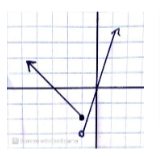
\includegraphics[width=\textwidth]{imgs/ex1.png}
\end{minipage}
\hspace{0.05\textwidth}
\begin{minipage}{0.6\textwidth}
    $\text{1. Given that}$
    $$f(x)=\left\{\begin{array}{c}
    -x-3, x \leq 1 \\
    3 x, x>-1
    \end{array}\right\},$$
    $\text{use a graphing approach to determine} \lim\limits_{x \to -1} f(x)$ or justify that it does not exist.
    $\lim_{x \to -1^-}f(x)=-2$\\
    $\lim_{x\ to -1^+}f(x)=-3$\\
   $\boxed{\therefore\ \lim\limits_{x \to -1} f(x)\text{ does not exist}}$
    \vspace{1cm}
\end{minipage}
Evaluate the following using a graphing approach:
\[
\lim_{x \to 2}\left(\sqrt{x-2}+3\right)
\]
\noindent
\begin{minipage}[t]{0.5\textwidth}
    \vspace{0pt}
    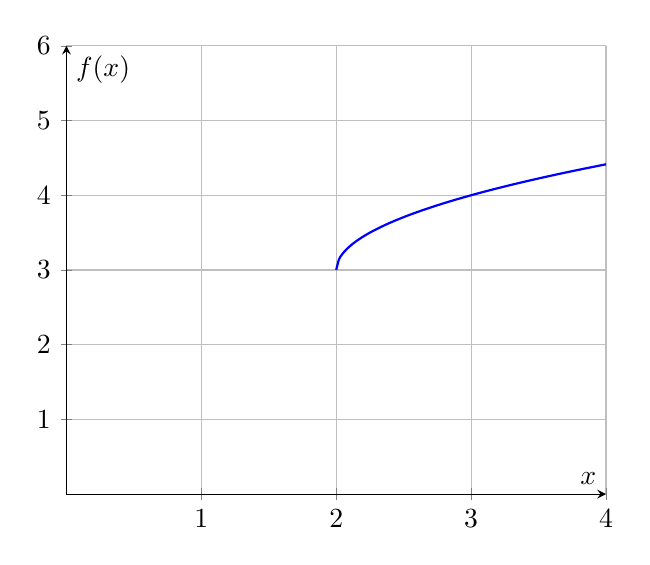
\begin{tikzpicture}
        \begin{axis}[
            xlabel=$x$,
            ylabel={$f(x)$},
            axis lines=middle,
            xmax=4,
            ymax=6,
            xmin=0,
            ymin=0,
            xtick={0,1,...,4},
            ytick={0,1,...,6},
            grid=both,
            domain=2:4,
            samples=100,
            smooth,
            legend pos=north west,
        ]
            \addplot[blue,thick] {sqrt(x-2) + 3};
        \end{axis}
    \end{tikzpicture}
\end{minipage}
\hfill
\begin{minipage}[t]{0.4\textwidth}
    \vspace{0pt}
    \begin{align*}
        \lim_{x \to 2^-}\left(\sqrt{x-2}+3\right) &= 3 \\
        \therefore \lim_{x \to 2}\left(\sqrt{x-2}+3\right) &= 3
    \end{align*}
\end{minipage}
\newpage 
\subsection{Limits as x goes to Negative infinity or Infinity}
We previously discussed how to evaluate limits as x goes to infinity or as x goes to negative infinity using a graphing approach.\\
However, we can discuss how to evaluate these types of limits without using a graphing approach every time.\\
To discuss how to do this, we will look at some graphs.
It is NOT important to know the numbers of the scenarios that follow.

\subsubsection{Scenario 1}
\begin{minipage}[t]{0.5\textwidth}
    \vspace{0pt}
    Suppose $y=a^x, 0 <a<1$\\
    For example, suppose $y=\left(\frac{1}{2}\right)^x$\\
    $\lim_{x \to -\infty}f(x)=\infty$\\
    $\lim_{x \to \infty}f(x)=0$
\end{minipage}
\begin{minipage}[t]{0.45\textwidth}
    \vspace{0pt}
    \begin{tikzpicture}[scale=0.8]
        \draw[->] (-3,0) -- (3,0) node[below] {$x$};
        \draw[->] (0,-1) -- (0,3) node[left] {$f(x)$};
        \draw[domain=-2:3,smooth,variable=\x,blue] plot ({\x},{0.5^\x});
        \draw[dashed] (-3,2) -- (3,2) node[right] {$1$};
        \draw[dashed] (-2,0) -- (-2,0.5) node[above] {$a$};
    \end{tikzpicture}
\end{minipage}

\subsubsection{Scenario 2}
\begin{minipage}[t]{0.5\textwidth}
    \vspace{0pt}
    Suppose $y=a^x, a>1$\\
    For example, suppose $y=2^x$\\
    $\lim_{x \to -\infty}f(x)=0$\\
    $\lim_{x \to \infty}f(x)=\infty$
\end{minipage}
\begin{minipage}[t]{0.45\textwidth}
    \vspace{0pt}
    \begin{tikzpicture}[scale=0.8]
        \draw[->] (-3,0) -- (3,0) node[below] {$x$};
        \draw[->] (0,-1) -- (0,3) node[left] {$f(x)$};
        \draw[domain=-2:2,smooth,variable=\x,blue] plot ({\x},{2^\x});
        \draw[dashed] (-3,1) -- (3,1) node[right] {$1$};
        \draw[dashed] (-2,0) -- (-2,2) node[above] {$a$};
    \end{tikzpicture}
\end{minipage}

\subsubsection{Scenario 3}
\begin{minipage}[t]{0.5\textwidth}
    \vspace{0pt}
    Suppose $y=a^x, a=1$\\
    $\lim_{x \to -\infty}f(x)=1$\\
    $\lim_{x \to \infty}f(x)=1$
\end{minipage}
\begin{minipage}[t]{0.45\textwidth}
    \vspace{0pt}
    \begin{tikzpicture}[scale=0.8]
        \draw[->] (-3,0) -- (3,0) node[below] {$x$};
        \draw[->] (0,-1) -- (0,3) node[left] {$f(x)$};
        \draw[domain=-3:3,smooth,variable=\x,blue] plot ({\x},{1^\x});
        \draw[dashed] (-3,1) -- (3,1) node[right] {$1$};
        \draw[dashed] (-2,0) -- (-2,1) node[above] {$a$};
    \end{tikzpicture}
\end{minipage}

\subsubsection{Scenario 4}
\begin{minipage}[t]{0.5\textwidth}
    \vspace{0pt}
    Suppose $y=x^a, a>0$\\
    $\lim_{x \to \infty}f(x)=\infty$
\end{minipage}
\begin{minipage}[t]{0.45\textwidth}
    \vspace{0pt}
    \begin{tikzpicture}[scale=0.8]
        \draw[->] (0,0) -- (3,0) node[below] {$x$};
        \draw[->] (0,0) -- (0,3) node[left] {$f(x)$};
        \draw[domain=0.1:3,smooth,variable=\x,blue] plot ({\x},{\x});
        \draw[dashed] (0,0) -- (3,3) node[right] {$x^a$};
    \end{tikzpicture}
\end{minipage}

\subsubsection{Scenario 5}
\begin{minipage}[t]{0.5\textwidth}
    \vspace{0pt}
    Suppose $y=x^a, a<0$\\
    For example, suppose $y=x^{-1/2}$ or $y=-2$\\
    $\lim_{x \to \infty}x^a=0$
\end{minipage}
\begin{minipage}[t]{0.45\textwidth}
    \vspace{0pt}
    \begin{tikzpicture}[scale=0.8]
        \draw[->] (0,0) -- (3,0) node[below] {$x$};
        \draw[->] (0,0) -- (0,3) node[left] {$f(x)$};
        \draw[domain=0.3:3,smooth,variable=\x,blue] plot ({\x},{1/\x});
        \draw[dashed] (0,0) -- (3,0) node[right] {$x^a$};
    \end{tikzpicture}
\end{minipage}

\subsubsection{Scenario 6}
\begin{minipage}[t]{0.5\textwidth}
    \vspace{0pt}
    Suppose $y=a^x, a=0$\\
    $\lim_{x \to \infty}f(x)=1$
\end{minipage}
\begin{minipage}[t]{0.45\textwidth}
    \vspace{0pt}
    \begin{tikzpicture}[scale=0.8]
        \draw[->] (0,0) -- (3,0) node[below] {$x$};
        \draw[->] (0,0) -- (0,3) node[left] {$f(x)$};
        \draw[domain=0:3,smooth,variable=\x,blue] plot ({\x},{1});
        \draw[dashed] (0,1) -- (3,1) node[right] {$a^x$};
    \end{tikzpicture}
\end{minipage}

\newpage
\textbf{\underline{Limits of Rational Functions as \( x \) Approaches Infinity or Negative Infinity:}}

When evaluating the limit of a rational function as \( x \) approaches either infinity or negative infinity (i.e., a polynomial over another polynomial), the following approach can be employed:

\begin{enumerate}
    \item Determine the degrees of the numerator and denominator. Factor out \( x^n \) from both the numerator and denominator, where \( n \) is the greater or lesser of the two degrees. If both degrees are the same, \( n \) equals that degree. (Factor out the same term from both the numerator and denominator.) Cancel out like factors.
    
    \item Determine the limit of each term in the numerator and sum those limits. Determine the limit of each term in the denominator and sum those limits.
    \begin{enumerate}
        \item A numerator with a finite limit over a denominator growing without bound yields a limit of 0.
        
        \item A numerator with a finite limit over a denominator with a finite limit produces a limit equal to the quotient of those limits.
        
        \item A numerator with a finite limit over a denominator that tends to zero yields a limit of infinity or negative infinity.
        
        \item A numerator growing without bound over a denominator that's finite or tends to zero produces a limit of infinity or negative infinity.
        
        \item A numerator that tends to zero over a denominator that's finite or growing without bound yields a limit of 0.
    \end{enumerate}
\end{enumerate}
\subsection{Continuity}

The idea of continuity can be thought of informally as the idea of being able to draw a graph without lifting one’s pencil.\\
Three types of discontinuity are illustrated below.

\begin{figure}[h]
\centering
\begin{minipage}{0.3\textwidth}
\centering
\begin{tikzpicture}[scale=0.8]
  % Axes
  \draw[->] (-1.5,0) -- (1.5,0) node[right] {$x$};
  \draw[->] (0,-1.5) -- (0,1.5) node[above] {$y$};
  
  % Hole
  \draw[fill=white] (0.75,0.75) circle [radius=0.03];
  \draw[dashed] (0.75,0.75) circle [radius=0.03];
  
  % Labels
  \node[below right] at (0.75,0.75) {$\circ$ Hole};
\end{tikzpicture}
\caption*{Graph with a Hole}
\end{minipage}%
\hfill
\begin{minipage}{0.3\textwidth}
\centering
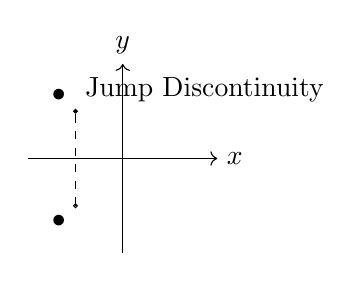
\begin{tikzpicture}[scale=0.8]
  % Axes
  \draw[->] (-1.5,0) -- (1.5,0) node[right] {$x$};
  \draw[->] (0,-1.5) -- (0,1.5) node[above] {$y$};
  
  % Jump Discontinuity
  \draw[fill=white] (-0.75,-0.75) circle [radius=0.03];
  \draw[fill=black] (-0.75,0.75) circle [radius=0.03];
  \draw[dashed] (-0.75,-0.75) -- (-0.75,0.75);
  
  % Labels
  \node[below left] at (-0.75,-0.75) {$\bullet$};
  \node[above left] at (-0.75,0.75) {$\bullet$};
  \node[above right] at (-0.75,0.75) {Jump Discontinuity};
\end{tikzpicture}
\caption*{Graph with a Jump Discontinuity}
\end{minipage}%
\hfill
\begin{minipage}{0.3\textwidth}
\centering
\begin{tikzpicture}[scale=0.8]
  % Axes
  \draw[->] (-1.5,0) -- (1.5,0) node[right] {$x$};
  \draw[->] (0,-1.5) -- (0,1.5) node[above] {$y$};
  
  % Vertical Asymptote
  \draw[dashed] (1,-1.5) -- (1,1.5);
  
  % Labels
  \node[above right] at (1,1.5) {Vertical Asymptote};
\end{tikzpicture}
\caption*{Graph with a Vertical Asymptote}
\end{minipage}
\end{figure}
\[
\boxed{\text{The function } f \text{ is continuous at } x=a \text{ if } f(a) \text{ is defined and if } f(a) = \lim_{x\to a} f(x)}
\]

\subsection*{Discontinuities}


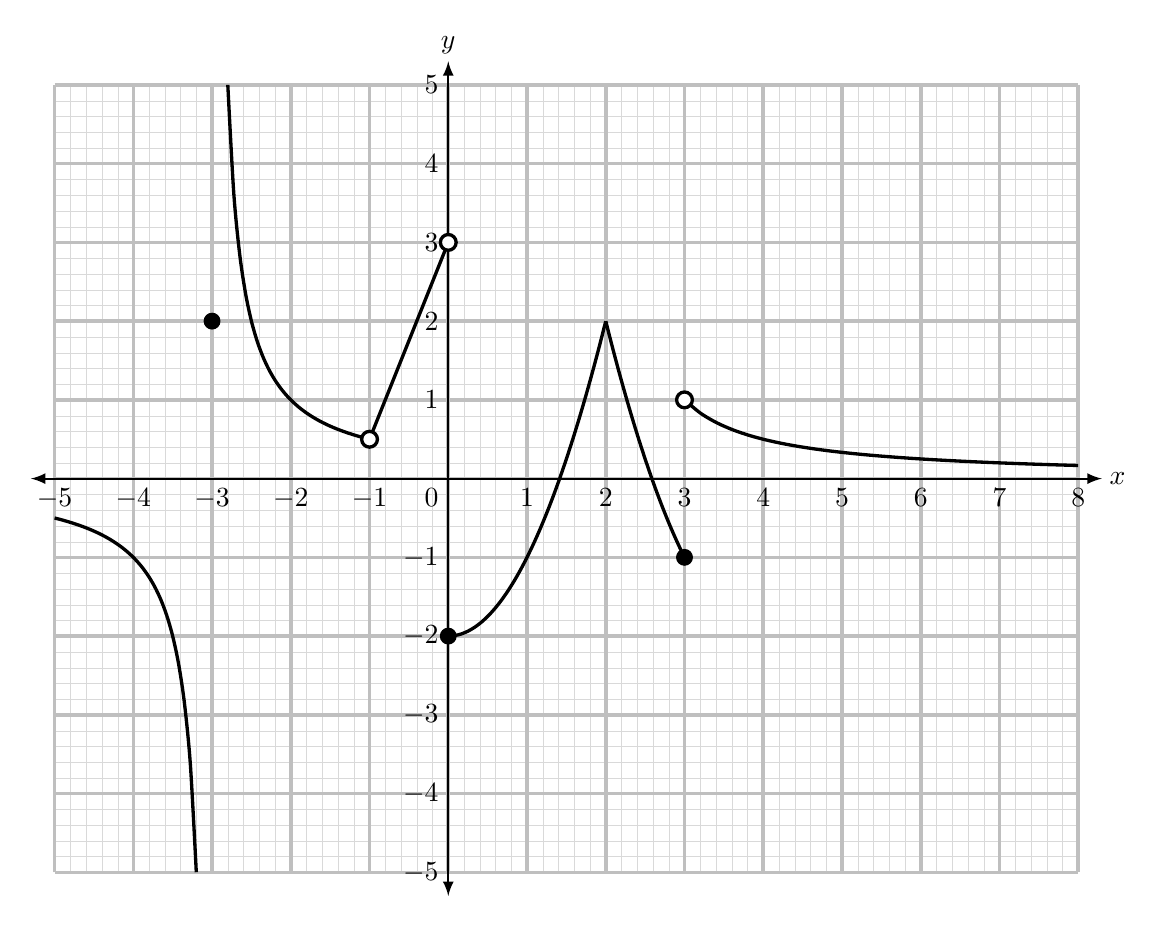
\begin{tikzpicture} 
    \def \minx {-5}
    \def \maxx {8}
    \def \miny {-5}
    \def \maxy {5}


    \draw[black!15, line width=0.05pt,  step=0.2] (\minx,\miny) grid (\maxx,\maxy);
    \draw[black!25, line width=1.3pt, step=1] (\minx,\miny) grid (\maxx,\maxy);


    \draw[thick, latex-latex] (\minx-0.3,0)--(\maxx+0.3,0);
    \draw[thick, latex-latex] (0,\miny-0.3)--(0,\maxy+0.3);
    \node at (\maxx+0.5,0) {$x$};
    \node at (0,\maxy+0.5) {$y$};

    \foreach \x in {\minx,...,-1}
     \node[below,black] at (\x,0) {$\x$};
    \foreach \x in {1,2,...,\maxx}
     \node[below,black] at (\x,0) {$\x$};
    \foreach \y in {\miny,...,-1}
     \node[left,black] at (0,\y) {$\y$};
    \foreach \y in {1,2,...,\maxy}
     \node[left,black] at (0,\y) {$\y$};
    \node[below left,black] at (0,0) {$0$};

    \draw[very thick, domain=-5:-3.2, smooth,variable=\x]  plot ({\x},{1/(\x+3)});
    \draw[very thick, domain=-2.8:-1, smooth,variable=\x]  plot ({\x},{1/(\x+3)});
    \draw[very thick, domain=-1:0, smooth,variable=\x]  plot ({\x},{2.5*\x+3});
    \draw[very thick, domain=0:2, smooth,variable=\x]  plot ({\x},{\x*\x - 2});
    \draw[very thick, domain=2:3, smooth,variable=\x]  plot ({\x},{(\x-4)*(\x-4) - 2});
    \draw[very thick, domain=3:8, smooth,variable=\x]  plot ({\x},{1/(\x-2)});

    \draw [very thick,fill=white] (0,3) circle [radius=0.1];
    \draw [very thick,fill=white] (3,1) circle [radius=0.1];
    \draw [very thick,fill=white] (-1,.5) circle [radius=0.1];
    \draw [fill] (0,-2) circle [radius=0.1];
    \draw [fill] (3,-1) circle [radius=0.1];
  	\draw [fill] (-3,2) circle [radius=0.1];
\end{tikzpicture}




\subsubsection{General Observations Regarding Continuity:}
\begin{enumerate}
    \item A function that is not continuous has some type of break in its graph.  This break is the result of a hole, jump, or vertical asymptote.
\item All polynomial functions are continuous for all real numbers.
\item A rational function $h(x)=\frac{f(x)}{g(x)}$is continuous at $x=a$ if $g(a)\neq 0$
\item A rational function in simplified for has a discontinuity at the zeros of the denominator.
\item When the one-sided limits are not equal to each other, then the limit at this point does not exist and the function is not continuous at this point
\end{enumerate}
\newpage 

\subsection{Properties of Limits}
\begin{itemize}
\item 1) $\lim _{x \rightarrow a} x=a$ \\
\item 2) $\lim _{x \rightarrow a} c=c$ \\
\item 3) $\lim _{x \rightarrow a}[c f(x)]=c \lim _{x \rightarrow a} f(x)$ \\
\item 4) $\lim _{x \rightarrow a}[f(x) \pm g(x)]=\lim _{x \rightarrow a} f(x) \pm \lim _{x \rightarrow a} g(x)$\\
\item 5) $\lim _{x \rightarrow a}[f(x) g(x)]=\lim _{x \rightarrow a} f(x) \lim _{x \rightarrow a} g(x)$\\
\item 6) $\lim _{x \rightarrow a} \frac{f(x)}{g(x)}=\frac{\lim _{x \rightarrow a} f(x)}{\lim _{x \rightarrow a} g(x)}$, only if $\lim _{x \rightarrow a} g(x) \neq 0$\\
\item 7) $\lim _{x \rightarrow a}[f(x)]^n=\left[\lim _{x \rightarrow a} f(x)\right]^n$\\

\item Where $\mathrm{c}$ is a constant, $\lim _{x \rightarrow a} f(x)$ and $\lim _{x \rightarrow a} g(x)$ exist.\\

\item If $P(x)$ is a polynomial, then
$$\lim _{x \rightarrow a} P(x)=P(a)$$
\end{itemize}
\newpage
\section{Unit 2 - Derivatives}
\subsection{Instantaneous Rate of Change, aka Tangent Lines, Slope at a Point, Derivatives}
\underline{Tangent Lines:} A tangent line to a curve is the straight line that most resembles the graph near that point.  By finding the slope of a tangent line, we can find the slope of the curve at the given point. \\ \\ 
Here are some examples of tangent lines:

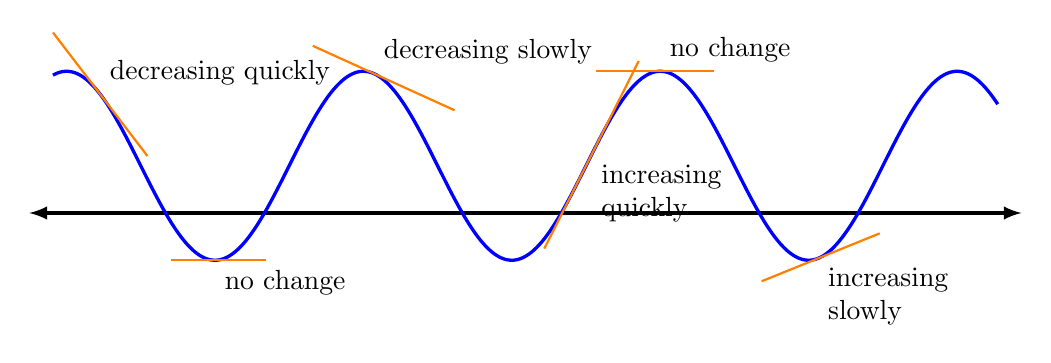
\begin{tikzpicture}[scale=0.6]
  \draw[latex-latex, very thick] (-5.5,0)--(15.5,0);

  \draw[domain=-5:15,samples=200,smooth,variable=\x, blue, very thick] plot ({\x},{1+2*sin(\x r)});
 
  \draw[domain=-5:-3,smooth,variable=\x, orange, thick] plot ({\x},{2*\x*cos(4 r) + 1 - 2*sin(4 r) + 8*cos(4 r)});
  \node[above right] at (-4,{1+2*sin(-4 r)}) {decreasing quickly};
 
  \draw[domain=-2.5:-.5,smooth,variable=\x, orange, thick] plot ({\x},{1+2*sin(-1.57 r)});
  \node[below right] at (-1.57,{1+2*sin(-1.57 r)}) {no change};
 
  \draw[domain=0.5:3.5,smooth,variable=\x, orange, thick] plot ({\x},{3.76562-0.4544*\x});
  \node[above right] at (1.8,{1+2*sin(1.8 r)}) {decreasing slowly};
 
  \draw[domain=5.4:7.4,smooth,variable=\x, orange, thick] plot ({\x},{1.98637*\x - 11.4797});
  \node[below right,text width=2cm] at (6.4,{1+2*sin(6.4 r)}) {increasing quickly};
 
  \draw[domain=6.5:9,smooth,variable=\x, orange, thick] plot ({\x},{1+2*sin(7.85 r)});
  \node[above right] at (7.85,{1+2*sin(7.85 r)}) {no change};
 
  \draw[domain=10:12.5,smooth,variable=\x, orange, thick] plot ({\x},{0.40601*\x - 5.50566});
  \node[below right,text width=2cm] at (11.2,{1+2*sin(11.2 r)}) {increasing slowly};
\end{tikzpicture}
Up until now, we have talked about needing two points to determine the slope of a line. However, as we begin talking about derivatives, we need to talk about the slope of a curve at a certain point. \\
Suppose that we wish to determine the slope of the curve $y=f(x)$ at the point where $x=a$. This is the same as finding the slope of the line tangent to the curve $y=f(x)$ at $x=a$.\\
When $x=a$, $y=f(x)$.  Therefore, we will be trying to determine the slope of the curve $y=f(x)$ at the point $(a, f(a))$.

\begin{center}
    
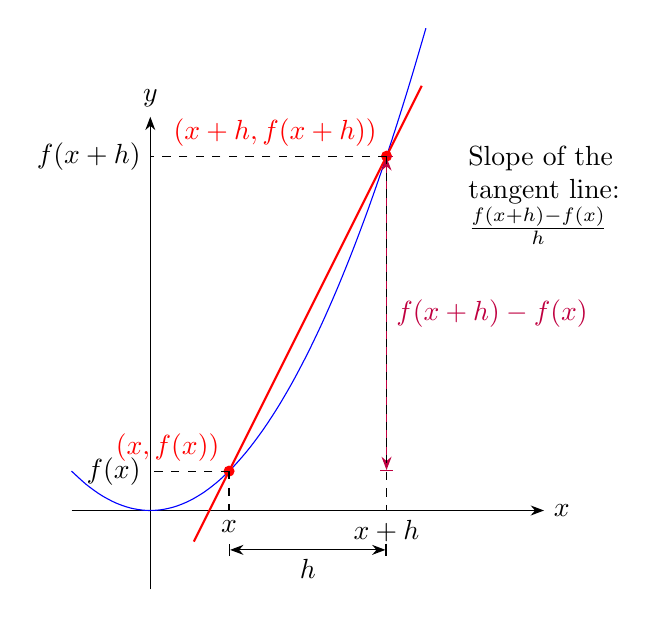
\begin{tikzpicture}[>=Stealth]
  \draw[->] (-1,0) -- (5,0) node[right] {$x$};
  \draw[->] (0,-1) -- (0,5) node[above] {$y$};
  
  \draw[scale=1,domain=-1:3.5,smooth,variable=\x,blue] plot ({\x},{0.5*\x*\x});
  
  \fill[red] (1,{0.5*1*1}) circle (2pt) node[above left] {$(x, f(x))$};
  \fill[red] (3,{0.5*3*3}) circle (2pt) node[above left] {$(x+h, f(x+h))$};
  
  \draw[red, thick, shorten <=-1cm,shorten >=-1cm] (1,{0.5*1*1}) -- (3,{0.5*3*3});
  
  \draw[|<->|] (1,-0.5) -- node[below] {$h$} (3,-0.5);
  
  \draw[|<->|,purple] (3,{0.5*3*3}) -- node[right] {$f(x+h)-f(x)$} (3,{0.5*1*1});
  
  \draw[dashed] (1,{0.5*1*1}) -- (1,0) node[below] {$x$};
  \draw[dashed] (3,{0.5*3*3}) -- (3,0) node[below] {$x+h$};
  \draw[dashed] (3,{0.5*3*3}) -- (0,{0.5*3*3}) node[left] {$f(x+h)$};
  \draw[dashed] (1,{0.5*1*1}) -- (0,{0.5*1*1}) node[left] {$f(x)$};

  \node at (5,4) [align=left] {Slope of the \\ tangent line:\\ $\frac{f(x+h)-f(x)}{h}$};
  
\end{tikzpicture}
\end{center}
    
\begin{tcolorbox}[colback=Orchid!5!white,colframe=Orchid!75!white,coltitle=white,title=Slope of Tangent ]
The derivative of the function $y=f(x)$ is given formula
  \[
  f'(x)=\lim_{h \to 0} \frac{f(x+h)-f(x)}{h},
  \]
 Other symbols for the derivative include $y'$ and $\frac{\delta y}{\delta x}$
\end{tcolorbox}
The derivative of a function allows you to determine the slope of the line tangent to a curve at a given point. In other words, you can find the slope of the line when you only know one point on the line. The value of the derivative is often called the instantaneous rate of change.
\subsubsection*{Example:}
Determine the derivative of the function $y=x^2$ and evaluate the derivative at the point where $x=3$.\\ \\ 
\textbf{Solution:}
\begin{align*}
    y' &= \lim_{x \to 0} \frac{f(x+h)-f(x)}{h}\\
    &= \lim_{h \to 0} \frac{(x+h)^2-x^2}{h}\\
    &= \lim_{h \to 0} \frac{x^2+2xh+h^2)-x^2}{h}\\
    &= \lim_{h \to 0} \frac{2xh+h^2}{h}\\
    &= \lim_{h \to 0} (2x+h)\\
    &= 2x + 0\\
    &= 2x.\\
    & \therefore y'=2x, \text{ at } x=3. \\
    y' &=2(3)=6 
\end{align*}
By evaluating the limit as the change in \( x \) approaches zero, we find the derivative \( y' = 2x \). Therefore, at \( x = 3 \), the derivative equals 6.
\newpage
\subsubsection*{Example:}
Determine the equation of the tangent line to the curve $y=x^2$ at the point where $x=3$. \\ \\ 
\textbf{Solution:}
\begin{align*}
    y &= mx + b, \quad \text{we know } m = 6 \\
    y &= 6x + b \\
    & \text{Substitute }(3, 9): \\
    9 &= 6(3) + b \\
    -9 &= b \\
\end{align*}
Therefore, the equation of the tangent at \(x = 3\) is \(y = 6x - 9\).
\subsubsection*{Example:}
Give that $y=3x^2-7x+6$, determine the value of $\frac{\delta y}{\delta x}$ at $x=5$. \\ \\ 
\textbf{Solution:}
\begin{align*}
    f'(x)&=\lim_{h to 0} \frac{f(x+h)-f(x)}{h}\\
    &=\lim_{h to 0} \frac{3(x+h)^2-7(x+h)+6-(3x^2-7x+6)}{h}\\
    &=\lim_{h to 0} \frac{3(x^2+2xh+h^2)-7x+7h+6-3x^2+7x-6}{h}\\
    &=\lim_{h to 0} \frac{\cancel{3x^2}+6xh+3h^2\cancel{-7x}+7h\cancel{+6}\cancel{-3x^2}\cancel{+7x}\cancel{-6}}{h}\\
    &= \lim_{h to 0} \frac{6hx+3h^2-7h}{h}\\
    &= \lim_{h to 0} \frac{\cancel{h}(6x+3h-7)}{\cancel{h}}\\
    &=6x+3(0)-7\\
    &= 6x-7
\end{align*}
At $x=5$ 
\begin{align*}
    &\frac{\delta y}{\delta x}=6(5)-7\\
    &=23
\end{align*}
\newpage
\subsubsection*{Example:}
Determine the equation of the tangent line of the curve $f(x)= \frac{1}{x}$ at the point where $x=2$.\\ \\ 
\textbf{Solution:}
\begin{align*}
    f'(x) &=\lim_{h \to 0}\frac{f(x+h)-f(x)}{h}\\
    &=\lim_{h \to 0}\frac{\frac{1}{x+h}-\frac{1}{x}}{h}\\
    &=\lim_{h \to 0} \frac{\frac{x}{x(x+h)} -\frac{(x+h)}{x(x+h)}}{h}\\
    &=\lim_{h \to 0} \frac{x-(x+h)}{xh(x+h)}\\
    &=\lim_{h \to 0} \frac{x-x-h}{xh(x+h)}\\
    &=\lim_{h \to 0} \frac{\cancel{h}}{x\cancel{h}(x+h)}\\
    &=\frac{-1}{x(x+0)}\\
    &=\frac{-1}{x^2}
\end{align*}
At $x=3$, $y=\frac{1}{2}$. Therefore, the point is $\left(2,\frac{1}{2}\right)$.\\
The derivative is $\frac{-1}{x^2}$. Therefore, the slope at $x=2$ is $\frac{-1}{2^2}=\frac{-1}{4}$
\begin{align*}
    &= y=mx+b\\
    &= y=\frac{-1}{4}x+b\\
    & \text{Sub in} \left(2,\frac{1}{2}\right)\\
    \frac{1}{2} &= \frac{-1}{4}(2)+b\\
    1 &=b
\end{align*}
The equation of the tangent line is $y=-\frac{1}{4}x+1$
\newpage 
\subsubsection*{Example:}
Determine an equation of the line that is perpendicular to the tangent to the graph of $f(x)=\frac{1}{x}$ at the point where $x=2$ and that intersects it at the point of tangency.(this is called the normal) \\  \\ 
\textbf{Solution:}

Our point is still $\left(2,\frac{1}{2}\right)$, our perpendicular slope is the negative reciprocal of the $-1\frac{1}{4}$, which is 4.
\begin{align*}
    &\therefore y=4x+b\\
    &\text{sub in} \left(2,\frac{1}{2}\right)\\
    \frac{1}{2}&=4(2)+b\\
    \frac{-15}{2}&=b\\
\end{align*}
The equation of the normal is $y=4x-\frac{15}{2}$
\subsection*{The Existence of Derivatives:}
A function $f$ is said to be differentiable at $x=a$ if $f'(a)$ exists. At points where $f$ is not differentiable, we say that the derivative does not exist. Common ways for a derivative to not exist are shown.

\begin{figure}[h]
\centering
\begin{minipage}[b]{0.5\textwidth}
\centering
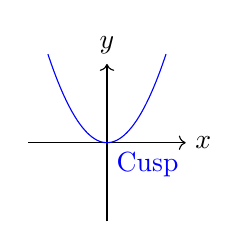
\begin{tikzpicture}[scale=0.5]
  % Cusp
  \draw[->] (-2,0) -- (2,0) node[right] {$x$};
  \draw[->] (0,-2) -- (0,2) node[above] {$y$};
  \draw[domain=-1.5:1.5, smooth, variable=\x, blue] plot ({\x}, {\x*\x});
  \node[below right, blue] at (0,0) {Cusp};
\end{tikzpicture}
\end{minipage}%
\begin{minipage}[b]{0.5\textwidth}
\centering
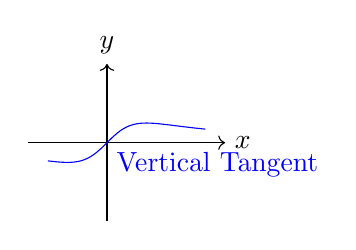
\begin{tikzpicture}[scale=0.5]
  % Vertical tangent
  \draw[->] (-2,0) -- (3,0) node[right] {$x$};
  \draw[->] (0,-2) -- (0,2) node[above] {$y$};
  \draw[domain=-1.5:2.5, smooth, variable=\x, blue] plot ({\x}, {\x/(1+\x*\x)});
  \node[below right, blue] at (0,0) {Vertical Tangent};
\end{tikzpicture}
\end{minipage}\\[20pt]
\begin{minipage}[b]{0.5\textwidth}
\centering
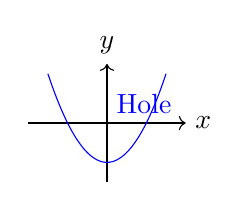
\begin{tikzpicture}[scale=0.5]
  % Hole
  \draw[->] (-2,0) -- (2,0) node[right] {$x$};
  \draw[->] (0,-1.5) -- (0,1.5) node[above] {$y$};
  \draw[domain=-1.5:1.5, smooth, variable=\x, blue] plot ({\x}, {(\x-1)*(\x+1)});
  \node[above right, blue] at (0,0) {Hole};
\end{tikzpicture}
\end{minipage}%
\begin{minipage}[b]{0.5\textwidth}
\centering
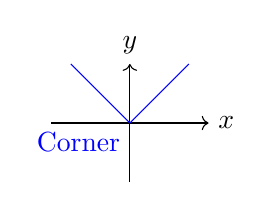
\begin{tikzpicture}[scale=0.5]
  % Corner
  \draw[->] (-2,0) -- (2,0) node[right] {$x$};
  \draw[->] (0,-1.5) -- (0,1.5) node[above] {$y$};
  \draw[domain=-1.5:1.5, variable=\x, blue] plot ({\x}, {abs(\x)});
  \node[below left, blue] at (0,0) {Corner};
\end{tikzpicture}
\end{minipage} 
\caption{Different Types of Discontinuities}
\label{fig:discontinuities}
\end{figure}


\section*{No Derivative}
\begin{minipage}[h]{0.7\textwidth}
  \centering
  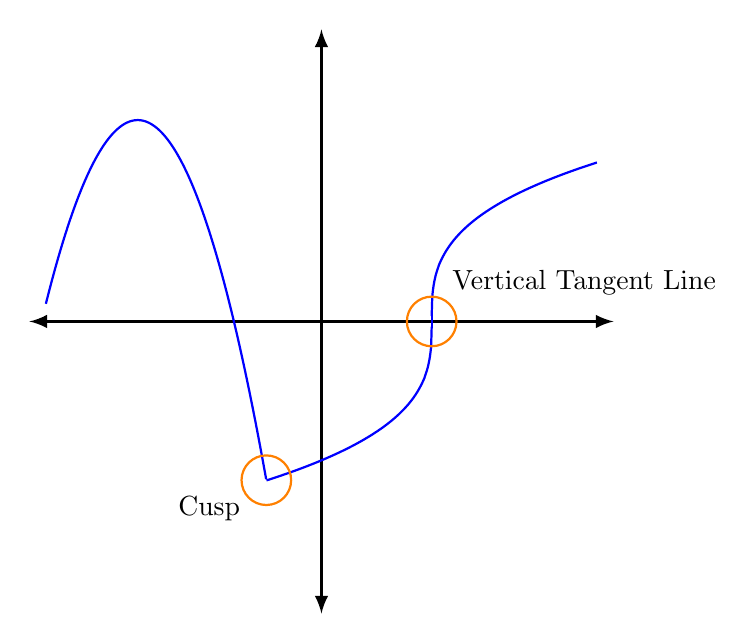
\begin{tikzpicture}[scale=0.7]
    \draw[latex-latex, very thick] (-5.3,0)--(5.3,0);
    \draw[latex-latex, very thick] (0,-5.3)--(0,5.3);
  
    \draw[domain=2.0001:5,samples=300,smooth,variable=\x, blue,  thick] plot ({\x},{2*exp(ln(\x-2)/3)});
    \draw[domain=2.0001:5,samples=300,smooth,variable=\x, blue,  thick,rotate around={180:(2,0)}] plot ({\x},{2*exp(ln(\x-2)/3)});
    \draw[blue,thick] (2,-0.1)--(2,0.1);
    \draw[domain=-5:-1,samples=300,smooth,variable=\x, blue,  thick] plot ({\x},-1.2*\x*\x-8*\x-9.68);
    \draw[orange,thick](-1,-2.88) circle (0.45);
    \draw[orange,thick](2,0) circle (0.45);
    \node[left] at (-1.3,-3.4) {Cusp};
    \node[above right] at (2.2,0.3) {Vertical Tangent Line};
  \end{tikzpicture}
\end{minipage}%
\begin{minipage}[t]{0.5\textwidth}
This graph represents a function that is not differentiable at certain points. The presence of a cusp and vertical tangent lines indicates that the function lacks a derivative at those points.
\end{minipage}

\section*{Inverse Derivative}
\begin{minipage}[h]{0.7\textwidth}
  \centering
  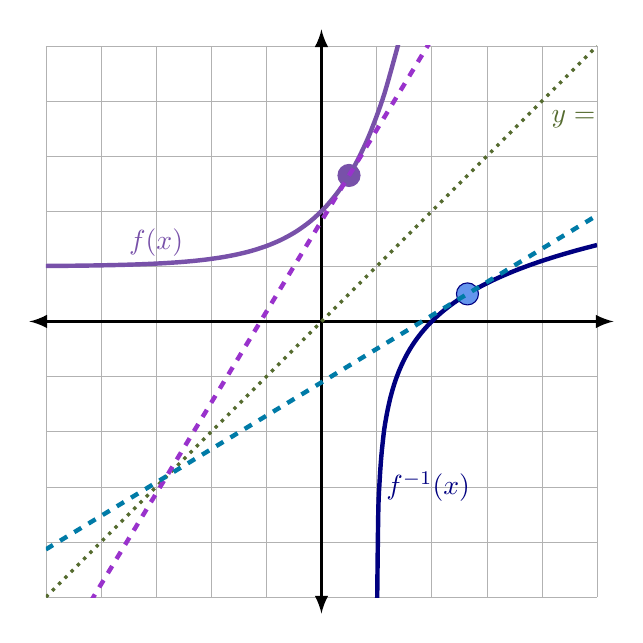
\begin{tikzpicture}[scale=0.7]
    \draw[black!30!white, very thin] (-5,-5) grid (5,5);
    \draw[latex-latex, very thick] (-5.3,0)--(5.3,0);
    \draw[latex-latex, very thick] (0,-5.3)--(0,5.3);
    
    \begin{scope}
        \clip (-5,-5) rectangle (5,5);
        \draw[very thick, OliveGreen,dotted](-5,-5)--(5,5);
        \node[OliveGreen,below right] at (4,4) {$y=x$};
        
        \draw[domain=-5:1.4,smooth,variable=\x, RoyalPurple, ultra thick] plot ({\x},{exp(\x)+1});
        \node[RoyalPurple,above] at (-3,1) {$f(x)$};
        \draw[RoyalPurple,fill=RoyalPurple] (0.5,2.649) circle [radius=0.2];
        \draw[domain=-4.5:2,smooth,variable=\x, DarkOrchid, ultra thick,dashed] plot ({\x},{1.649*\x+1.824});
        
        \draw[domain=1.003:5,smooth,variable=\x, NavyBlue, ultra thick, samples=150] plot ({\x},{ln(\x-1)});
        \node[NavyBlue,right] at (1,-3) {$f^{-1}(x)$};
        \draw[NavyBlue,fill=CornflowerBlue] (2.649,0.5) circle [radius=0.2];
        \draw[domain=-5:5,smooth,variable=\x, Cerulean, ultra thick,dashed] plot ({\x},{0.606*\x-1.105});
    \end{scope}
  \end{tikzpicture}
\end{minipage}%
  \vspace{2em}
\begin{minipage}[h]{0.5\textwidth}
This graph represents the inverse function of a function that has a derivative. The presence of a straight line indicates that the inverse function is linear. Additionally, the graph illustrates that the inverse function reverses the behavior of the original function with respect to the line $y=x$.
\end{minipage}



\subsection{Power Rule}
\begin{tcolorbox}[sharp corners=uphill,
    colback=purple!50!white,colframe=blue!25!black,coltext=yellow,
    fontupper=\Large\bfseries,arc=6mm,boxrule=2mm,boxsep=5mm]
  if $f(x)=x^{n}$, then $f'(x)=nx^{n-1}$
\end{tcolorbox}
  \textit{Proof}\\
  \begin{align*}
    f'(x)&=\lim_{h \to 0}\frac{f(x+h)-f(x)}{h}\\
    & \text{if } f(x)=x^n\\
    & \text{Then, } f(x+h)= (x+h)^n 
  \end{align*}
\subsubsection*{Example:}
if $f(x)= 4x^5$, then determine $f'(x)$. \\ \\ 
\textbf{Solution:}
\begin{align*}
    &= 4x^5\\
    &= (5)(4)x^{5-1}\\
    &=20x^4
\end{align*}
\subsubsection*{Example:}
if $f(x)= 11x^{\frac{5}{2}}$, then determine $f'(x)$.\\ \\ 
\textbf{Solution:}
\begin{align*}
    &= 11x^{\frac{5}{2}}\\
    &= \left(\frac{5}{2}\right)(10)x^{\frac{5}{2}-1}\\
    &= \frac{55}{2}x^{\frac{3}{2}}\\
\end{align*}
\subsubsection*{Example:}
if $f(x)=7x$, then determine $f'(x)$.\\ \\ 
\textbf{Solution:}
\begin{align*}
    &=(0)(7)x^{0-1}\\
    &=0
\end{align*}
\newpage
\subsection{Product Rule}
\begin{tcolorbox}[colback=Orchid!5!snow, colframe=nadeshikopink!50!white,
  colbacktitle=mordantred19!75!mistyrose, title=Product Rule]

The product rule states that if $p(x)=f(x)g(x)$, then\\ $p'(x)=f'(x)g(x)+f(x)g'(x)$.
\textbf{Product Rule in Newton Notation.}\\


$\frac{\delta}{\delta x}(uv)=\left(\frac{\delta u}{\delta x}\right)v+u\left(\frac{\delta v}{\delta x}\right)$
\textbf{Product Rule in Leibniz Notation}

\end{tcolorbox}
\textit{Proof of the Product Rule}
\begin{align*}
    p'(x) &= \lim_{h \to 0}\frac{p(x+h)-p(x)}{h}\\
    &=\lim_{h \to 0}\frac{f(x+h)g(x+h)-f(x)g(x)}{h}\\
    &=\lim_{h \to 0}\frac{f(x+h)g(x+h)\textcolor{red}{-f(x)g(x+h)+f(x)g(x+h)}-f(x)g(x)}{h}\\
    &= \lim_{h \to 0}\left[\frac{f(x+h)-f(x)}{h}\right]g(x+h)+f(x)\left[\frac{g(x+h)-g(x)}{h} \right]\\
    &=\left(\lim_{h \to 0} \frac{f(x+h)-f(x)}{h} \right) \left[\lim_{h \to 0}g(x+h)\right]+\left[\lim_{h \to 0} f(x)\right]\left(\lim_{h \to 0}\frac{g(x+h)-g(x)}{h}  \right)\\
    &=f'(x)g(x)+f(x)g'(x)
\end{align*}
\subsection*{Example}
Differentiate $h(x)=(x^3-2x)(3x^4+2x+8)$.\\
\textbf{Solution:}
$h'(x)=(3x^2-2)(3x^4+2x+8)+(x^3-2x)(12x^3+2)$.

Because of the power rule, we are able to say that the derivative of $kf(x)$ where is a scalar is $kf'(x)$.  In other words, we are able to just leave the scalar alone in front and determine the derivative of the function.\\
An example of this would be that if $y=7(3x^2+2x+6)$, then $$\frac{\delta y}{\delta x}=7(6x+2)$$\\
In other words, the derivative would equal 7 times the derivative of the polynomial.\\
How do we know this? By the power rule. Here’s the explanation.
Let $f(x)g(x)$, where $f(x)=7$ and $g(x)=3x^2+2x+6$.  

\begin{align}
    \frac{\delta y}{\delta x}&=f'(x)g(x)+f(x)g'(x)\\
    \frac{\delta y}{\delta x}&=(0)(3x^2+2x+6)+7(6x+2)\\
    &=7(6x+2)
\end{align}

\subsection{Quotient Rule}
"Low di high minus high di low over low low." \\
What does this mean? Well it means the quotient rule

\begin{tcolorbox}[colback=blue!5!snow, colframe=white!50!white,
  colbacktitle=blue!75!mistyrose, title=Quotient Rule]
if $h(x)=\frac{f(x)}{g(x)}$, then $h'(x)=\frac{f'(x)g(x)-f(x)g'(x)}{[g(x)]^2}, g \neq 0$\\
In Leibniz notation, $\frac{\delta }{\delta x}(\frac{u}{v})=\frac{\frac{\delta u}{\delta x}v- u\frac{\delta v}{\delta x}}{v^2}$
\end{tcolorbox}
\textit{Proof:}
\begin{align*}
    h(x)&=\frac{f(x)}{g(x)} \implies h(x)g(x)=f(x)\\
    & \therefore \text{by the product rule, } h'(x)g(x)+h(x)g'(x)=f(x)'\\
    &\implies h'(x)\cancel{g(x)}=\frac{f'(x)-h(x)g'(x)}{g(x)}\\
    &h'(x)=\frac{f'(x)-\left[\frac{f(x)}{g(x)}\right]g'(x)}{g(x)}\\
    &=\frac{f'(x)\left( \textcolor{red}{\frac{g(x)}{g(x)}}\right)-\frac{f(x)g'(x)}{g(x)}}{g(x)}\\
    &=\frac{\frac{f'(x)g(x)}{g(x)}-\frac{f(x)g'(x)}{g(x)}}{g(x)}\\
    &=\frac{f'(x)g(x)-f(x)g'(x)}{[g(x)]^2}
\end{align*}
\subsubsection*{Example:}
Determine the derivative of $h(x)=\frac{3x-4}{x^2+5}$.\\
\textbf{Solution:}
$h'(x)=\frac{(x^2+5)(3)-(3x+4)(4)}{(x^2+5)^ 2}$
\newpage 


\subsection{Chain Rule}
\begin{tcolorbox}[colback=OliveGreen!5!snow, colframe=white!50!white,
  colbacktitle=OliveGreen!75!mistyrose, title=Chain Rule]
The chain rule states 
if $h(x)=f \circ g(x)$, then $f'(g(x))g'(x)$ \\
$\frac{\delta y}{\delta x}=\frac{\delta y}{\delta u} \times \frac{\delta u}{\delta x}$
\end{tcolorbox}
\textit{Proof:}\\
\begin{align*}
\left[f(g(x)) \right]'&=\lim_{h \to 0} \frac{f(g(x+h)-f(g(x)))}{h}\\
&= \lim_{h \to 0} \left[ \frac{f(g(x+h)-f(g(x))}{\textcolor{red}{g(x+h)-g(x)}} \frac{\textcolor{red}{g(x+h)-g(x)}}{h}\right]\\
&=\lim_{h \to 0}\frac{f(g(x+h))-f(g(x))}{g(x+h)-g(x)} \lim_{h \to 0}\frac{g(x+h)-g(x)}{h}\\
&\boxed{\text{let k } = g(x+h)-g(x) \therefore \text{ as } h \to 0, k \to0}\\
&= \left[\lim_{\textcolor{red}{k \to 0}}\frac{f(g(x+\textcolor{red}{k})-f(g(x))}{\textcolor{red}{k}} \right]\left[ \lim_{h \to 0}\frac{g(x+h)-g(x)}{h}\right]\\
&=f'(g(x))g'(x)
\end{align*}
\subsubsection*{Example 1:}
Determine the derivative of $h(x)=(10x^3-7x^2+3x-9)^{14}$\\
\textbf{Solution:}
$h'(x)=14(10x^3-7x^2+3x-9)^{13}(30x^2-14x+3)$
\subsubsection*{Example 2:}
Suppose $f(12)=-7, g(3)=12, f'(12)=11$ and $g'(3)=9$. If $h(x)=f(g(x))$, then evaluate $h'(3)$.\\
\textbf{Solution:}
\begin{align*}
    h'(x)&=f(g(x))\\
    h'(3)&=f'(g(3))g(3)\\
    &=f'(12)(9)\\
    &=(11)(9)\\
    &=99
\end{align*}
\newpage 

\subsection{Derivatives Not in Terms of x:}
Every time that we state a rate of change, we state that rate of change with respect to something.\\
For instance, if we talk about speed, we are talking about distance with respect to time.\\
When we discuss slope on a Cartesian plane, we use the formula:
$$m=\frac{y_2-y_1}{x_2-x_1}$$
In other words, we talk about the change in y with respect x.\\
Similarly, when we determine a derivative(which is just an instantaneous rate of change, or slope at a point), we determine the derivative with respect to something. Usually, we derivative with respect to x. However, this isn't always case.\\

The definition of a derivative is 
$$f'(x)=\lim_{h \to 0}\frac{f(x+h)-f(x)}{h}$$
The derivative is the limit of the slope between two points on a relation as those two points get infinitely close together. Alternatively, then we could define the derivative $$f'(x)= \lim_{x \to a }\frac{f(x)-f(a)}{x-a}$$

\subsubsection*{Example 1:}
Suppose $y=3(2x^2+x+-1)^4$. Determine $\frac{\delta y}{\delta x}$.\\
\textbf{Solution:}
$\frac{\delta y}{\delta x}=12(2x^2+x-1)^3(4x+1)$
\subsubsection*{Example 2:}
Suppose $y=3(2x^3+x-1)^4$. Determine $\frac{\delta y}{d(2x^2+x-1)}$.\\
\textbf{Solution:}
\begin{align*}
    \text{ let w } &= (2x^2+x-1)^4\\
    y&=3w^4\\
    \frac{\delta y}{\delta x}&=12w^3\\
    \frac{\delta y}{d(2x^2+x-1)}&=12(2x^2+x-1)^3
\end{align*}

\begin{center}
\begin{figure}
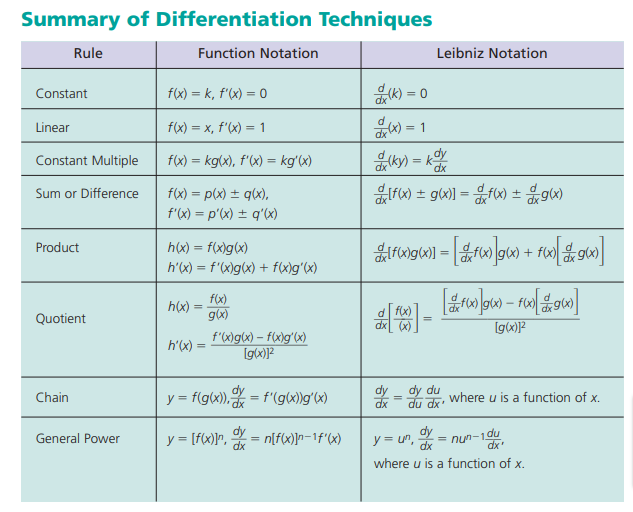
\includegraphics[width=1\textwidth]{imgs/summary of differentiation techniques.png}
\caption{Summary of Differentiation Techniques }
\end{figure}
\end{center}
\newpage 


\subsection{Implicit Differentiation}
Unit now, we have been determining derivatives when y is stated explicitly in terms of x.\\
However, sometimes are equation in terms of x, and remember to use the chain rule when differentiating terms containing y.\\
We may need to use other rules of differentiation as well.\\
\subsubsection{Intro to How Implicit Differentiation Works:}
\begin{itemize}
    \item The derivative pf $5x^3$ with respect to x is $15x^2$. We can think of this slightly differently though and say that the derivative of $5x^3$ with respect to x is $15x^2 \frac{\delta x}{\delta x}$ and that since $\frac{\delta x}{\delta x}=1$, therefore the derivative of $5x^3$ with respect to is $15x^2$
    \item By the same way of thinking, the derivative of $5y^3$ with respect to x is $15y^2 \frac{\delta y}{\delta x}$
\end{itemize}
\subsubsection*{Example}
If $x^2+y^2=25$, determine $\frac{\delta y}{\delta x}$ and determine the slope of the tangent to the curve at the point (3,-4).
\begin{align*}
    2x+2y \frac{\delta y}{\delta x}&=0\\
    2y \frac{\delta y}{\delta x}&=-2x\\
    \frac{\delta y}{\delta x}=\frac{-2x}{2y}\\
    \frac{\delta y}{\delta x}=\frac{-x}{y}\\
    \text{at }(3,-4), \frac{\delta y}{\delta x}&=\frac{-3}{-4}\\
    \frac{\delta y}{\delta x}=\frac{3}{4}
\end{align*}

\newpage 
\subsection{Related Rates}

\begin{itemize}
    \item After 1 second, the circular ripple would have an area of $\pi(1)^2=\pi m^2$ 
    \item After 2 seconds, the circular ripple would have an area of $\pi(2)^2=4\pi m^2$ (an increase of $3\pi m^2$)
    \item After 3 seconds, the circular ripple would have an area of $\pi(3)^2=9\pi m^2$ (an increase of $5\pi m^2$)
    \item After 4 seconds, the circular ripple would have an area of $\pi(4)^2=16\pi m^2$ (an increase of $7\pi m^2$)
\end{itemize}

We see that although the rate of increase of the radius remains constant, the rate of increase of the area is changing. The rate of increase of the area is related to the rate of increase of the radius. We call it a “related rate”. The rate of increase of the area is a function of time and it is not a constant.

Examples of Related Rates in Calculus
There are many types of related rates in Calculus. For example,
\begin{itemize}

\item Imagine a stone in a pond causing a circular ripple. The rate of increase of the area of the circular ripple will be related to the rate of increase of the radius of the ripple. If the rate of increase of the radius of the circular ripple is constant, the rate of increase of the area of the circular ripple will not be.

\item Imagine blowing air into a spherical balloon. The rate of increase of the radius of the sphere will be related to the rate of increase of the volume of the sphere. If the rate of increase of the volume of air in the sphere is constant, the rate of increase of the radius of the sphere will not be.

\item Imagine filling a cone shaped container with liquid. The rate of increase of the height of the liquid will be related to the rate of increase of the volume of the liquid in the cone. If the rate of increase of the volume of the liquid is constant, the rate of increase of the height of the liquid will not be.

There are many more examples.

\end{itemize}
\subsubsection{How To Approach a Related Rates Problem}
\begin{enumerate}
\item Some people like to draw a diagram.

\item Assign a variable to each quantity in the problem that is a function of the independent variable.  (We’ll assume for the remainder of this discussion that the independent variable is time)

\item Develop an equation that associates the variables with one another.4.Differentiate (possibly using implicit differentiation).

\item Substitute in given information and solve for the required rate of change.
\end{enumerate}
\subsubsection*{Example:} 
When a raindrop falls into a small puddle, it creates a circular ripple that spreads out from the point where the raundrop hit. The radius of the circle grows at a rate of 3 cm/s.
a) determine the rate of increase of the circumference of the circle with respect to time.\\
b) determine the rate of increase \\
\textbf{Solution:}

a) 
\begin{align*}
    \frac{\delta r}{dt}&=3\\
    C&=2\pi r\\
    \frac{\delta c }{\delta t}&=2 \pi \frac{\delta r}{\delta t}\\
    &=2 \pi (3cm/s)\\
    &=6 \pi cm/s 
\end{align*}
$\therefore$ the circumference increase at a rate of $6 \pi$ cm/s
b) 
\begin{align*}
    A&=\pi r^2\\
    \frac{\delta A}{\delta t} &=2\pi r \frac{\delta r}{\delta t}\\
    A&=81 \pi \\
    r^2&=81\\
    r&=9\\
    \frac{\delta A}{\delta t}&=2\pi (9 cm)(3cm/s)\\
    &=54\pi cm^2/s
\end{align*}

 
\subsubsection{How to approach each problem}
\begin{itemize}
    \item Identify the given variables and the quantities that need to be determined. Draw a picture if one is not given.

    \item Write an equation involving the rates whose variables are given or need to be determined. Do not substitute yet unless the value will never change.

    \item Using the chain rule, implicitly differentiate both sides of the equation with respect to time ($t$).

    \item Substitute into the resulting equation all known values for the variables and their rates of change. Then, solve for the required rate of change.	
\end{itemize}

\section{Unit 3}
\subsection{Higher Order Derivatives, Velocity, Acceleration, and Rates of Change}
\subsubsection*{Second Derivative Test}
The second derivative of $y=f(x)$ is the derivative of $y=f^{\prime}(x)$\\
In Newton notation, the second derivative is $f^{\prime \prime}(x)$\\
In Leibniz notation, the second derivative is $\frac{d^2 y}{d x^2}$\\

\underline{Displacement:} The position of an object with respect to time, usually referred to as $s(t)$.\\

\underline{Velocity:} The rate of change of displacement over time. Therefore, the first derivative of the displacement function with respect to time is velocity.\\
$$
v(t)=s^{\prime}(t) \quad \text { or } \quad v(t)=\frac{d s}{d t}
$$

\underline{Acceleration:} The rate of change of velocity over time. Therefore, the first derivative of the velocity function with respect to time, or the second derivative of displacement with respect to time, is acceleration.\\
$$
a(t)=v^{\prime}(t)=s^{\prime \prime}(t) \quad \text { or } \quad a(t)=\frac{d v}{d t}=\frac{d^2 s}{d t^2}
$$

\underline{Some Points to Ponder About Velocity and Acceleration}
\begin{itemize}
\item Negative velocity means that an object is moving in a negative direction (left or down) while positive velocity means the opposite
\item Zero velocity means that an object is stationary and that a possible change in direction may occur.
\item Negative acceleration means that the velocity is decreasing, while positive acceleration means that the velocity is increasing.
\item Zero acceleration means that the velocity is constant
\item The speed of an object is the magnitude of its velocity.
$$
\text {Speed }=|v(t)|=\left|s^{\prime}(t)\right|
$$
\item An object is speeding up (increasing speed) when its velocity and acceleration have the same signs. However, an object is slowing down (decreasing speed) when its velocity and acceleration have opposite signs.
\item If the displacement is measured in metres and time is measured in seconds, then velocity is measured in $\mathrm{m} / \mathrm{s}$ and the acceleration is measured in $\mathrm{m} / \mathrm{s}^2$.
\end{itemize}



\subsubsection*{Concavity}

We know that the sign of the derivative tells us whether a function is increasing or decreasing at some point. Likewise, the sign of the second derivative $f''(x)$ tells us whether $f'(x)$ is increasing or decreasing at $x$. We summarize the consequences of this seemingly simple idea in the table below:


\begin{figure}[ht]
    \centering
    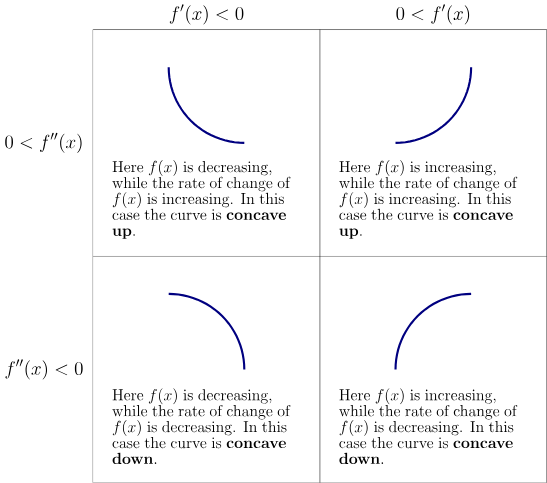
\includegraphics[width=0.7\textwidth]{imgs/digInConcavityAnd2ndDerivTest-figure0.png}
\end{figure}

The sign of the second derivative $f''(x)$ tells us about the behavior of the first derivative $f'(x)$:

\begin{center}
\begin{tabular}{@{}ll@{}}
\toprule
Sign of $f''(x)$ & Behavior of $f'(x)$ \\
\midrule
$f''(x) > 0$ & $f'(x)$ is increasing (concave up) \\
$f''(x) < 0$ & $f'(x)$ is decreasing (concave down) \\
\bottomrule
\end{tabular}
\end{center}



\newpage 

\subsubsection*{Example:}
\begin{center}
\begin{minipage}{\linewidth}
    \centering
    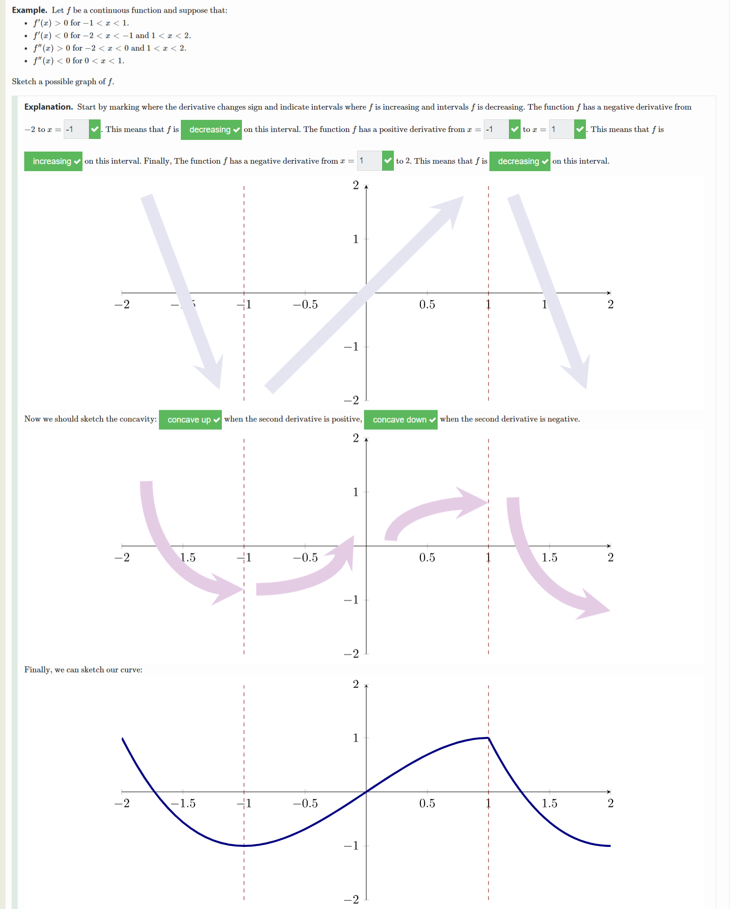
\includegraphics[width=1.3\textwidth]{imgs/ex.png}
\end{minipage}
\end{center}

\newpage 
\subsection{Inflection Points}
If we are trying to understand the shape of the graph of a function, knowing where it is concave up and concave down helps us to get a more accurate picture. Of particular interest are points at which the concavity changes from up to down or down to up.

\begin{tcolorbox}[sharp corners=uphill]
\underline{Definition:} If the concavity of $f$ changes either from up to down or down to up at $x=a$ and $f$ has a tangent line at $x=a$, then $x=a$ is an inflection point of $f$.
\end{tcolorbox}

It is instructive to see some examples of inflection points:

\begin{figure}[ht]
    \centering
    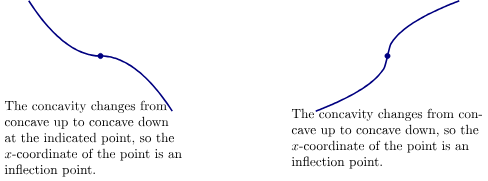
\includegraphics[width=0.7\textwidth]{imgs/digInConcavityAnd2ndDerivTest-figure4.png}
\end{figure}

\begin{figure}[ht]
    \centering
    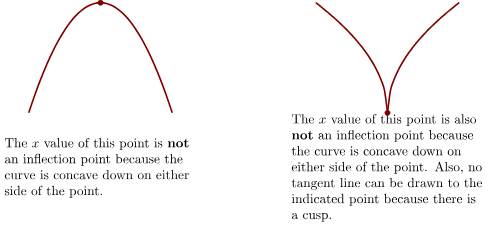
\includegraphics[width=0.7\textwidth]{imgs/digInConcavityAnd2ndDerivTest-figure5.png}
\end{figure}

\textcolor{red}{Warning:} Even if $f''(a)=0$, the point determined by $x=a$ might not be an inflection point. You also need to check that the concavity of $f$ changes on either side of $x=a$.
\newpage 

\subsubsection*{Example:}
\begin{center}
\begin{minipage}{\linewidth}
    \centering
    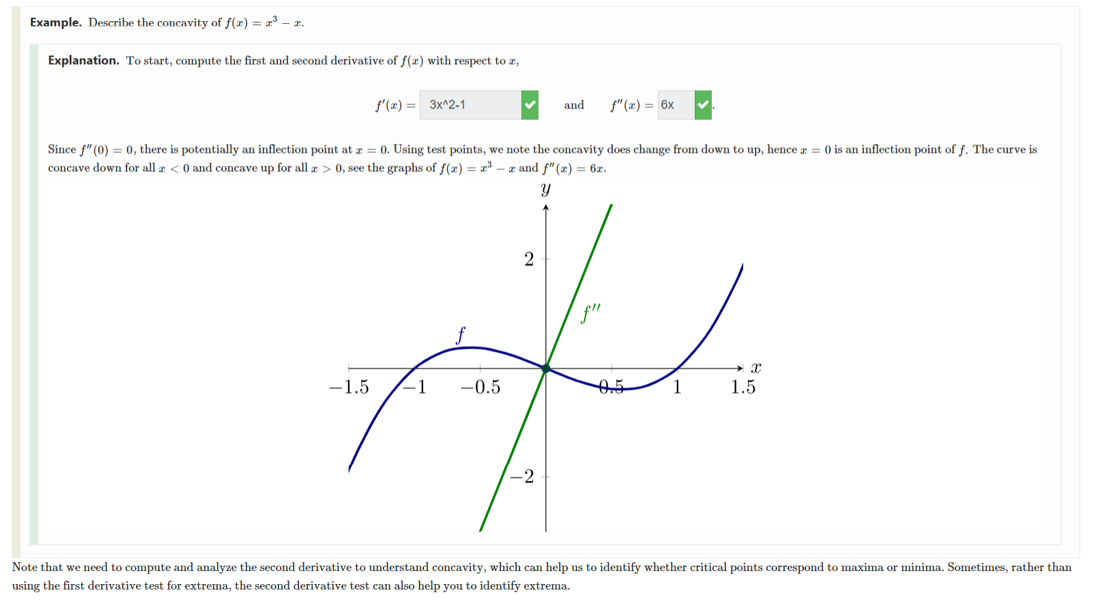
\includegraphics[width=1.3\textwidth]{imgs/ex3.png}
\end{minipage}
\end{center}
\underline{Problem:}
If $f''(a)=0$, what does the second derivative test tell us?


\begin{enumerate}
    \item[a)] The function has a local extrema at $x=a$
    \item[b)] The function does not have a local extrema at $x=a$
    \item[c)] It gives no information on whether $x=a$ is a local extremmum.
\end{enumerate}
The correct answer is C.
\subsubsection*{Example:}
\begin{center}
\begin{minipage}{\linewidth}
    \centering
    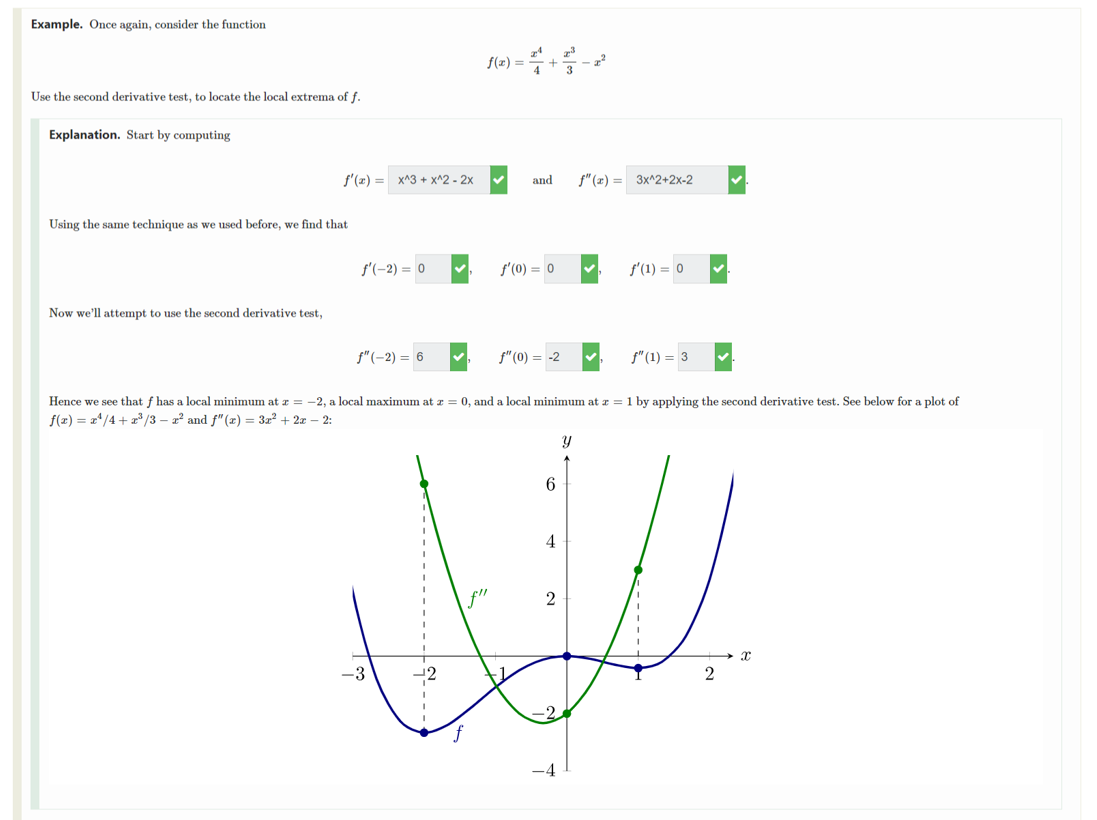
\includegraphics[width=1.3\textwidth]{imgs/ex4.png}
\end{minipage}
\end{center}
\underline{Second Derivative Test:}

\begin{itemize}
\item If $f'(c)=0$ and $f''(c)>0$, then there is a local minimum at $x=c$.
\item If $f'(c)=0$ and $f''(c)<0$, then there is a local maximum at $x=c$.
\item If $f'(c)=0$ and $f''(c)=0$, or if $f''(c)$ doesn't exist, then the test is inconclusive. There might be a local maximum or minimum, or there might be a point of inflection.
\end{itemize}
\newpage 
\subsection{Problem-Solving Strategy: Solving Optimization Problems}

\begin{enumerate}
    \item Introduce all variables. If applicable, draw a figure and label all variables.
    \item Determine which quantity is to be maximized or minimized, and for what range of values of the other variables (if this can be determined at this time).
    \item Write a formula for the quantity to be maximized or minimized in terms of the variables. This formula may involve more than one variable.
    \item Write any equations relating the independent variables in the formula from step 3. Use these equations to write the quantity to be maximized or minimized as a function of one variable.
    \item Identify the domain of consideration for the function in step 4 based on the physical problem to be solved.
    \item Locate the maximum or minimum value of the function from step 4. This step typically involves looking for critical points and evaluating a function at endpoints.
\end{enumerate}
You need to remember the surface area formulas from grade 8th math.
\begin{center}
\begin{minipage}{\linewidth}
    \centering
    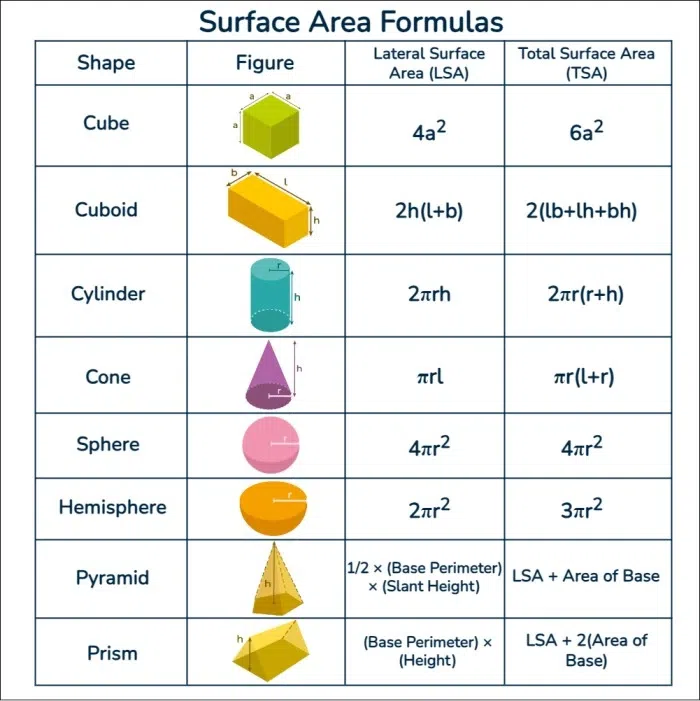
\includegraphics[width=0.8\textwidth]{imgs/Surface-Area-Formulas.png}
\end{minipage}
\end{center}
\newpage

\newpage
\section{Unit 5}
\subsection{Trig Derivatives }
The two main rules to remember are the following:
\begin{tcolorbox}[sharp corners=uphill,
    colback=purple!50!white,colframe=blue!25!black,coltext=yellow,
    fontupper=\Large\bfseries,arc=6mm,boxrule=2mm,boxsep=5mm]
$$\frac{\delta (\sin x)}{\delta x}=\cos x \quad \text{and } \quad \frac{\delta(\cos x)}{\delta}=-\sin x$$
\end{tcolorbox}
\textit{Proof} that $\frac{\delta (sin \theta)}{\delta x}=\cos \theta$.\\
We will do this proof in two parts. \\

In the first part, we will prove that  $\lim_{\theta \to 0}\left( \frac{\sin \theta }{\theta}\right)$\\

We need to prove this because it comes up within the main proof, which we will then do in part 2.\\

Part 1: Proving that $\lim_{\theta \to 0}\left( \frac{\sin \theta }{\theta}\right)$\\

Recall that the area of a circle is $\pi r^2=(\frac{2 \pi}{2})r^2$ \\
We will think of our angle $\theta$ in radians \\
The area of the sector of a circle created by a central angle of $\theta$ radians will represent $\frac{\theta}{2\pi}$ of the area of the circle as a whole \\

\begin{minipage}{0.5\textwidth}
For example, if the angle shown is $60^{\circ}$, or $\frac{\pi}{3}$ radians, then the area of the highlighted sector will represent $\left(\frac{\frac{\pi}{3}}{2\pi}\right)=\frac{\pi}{3}\times \frac{1}{2\pi}=\frac{\pi}{6\pi}=\frac{1}{6}$ of the area of the circle as a whole.
\end{minipage}
\hspace{1em}
\begin{minipage}{0.5\textwidth}
\begin{tikzpicture}[scale=2.5] 
\draw (0,0) circle (1cm);
\draw (0,0) -- (0:1cm); 
\draw (0,0) -- (60:1cm); 

\draw (0.2,0) arc (0:60:0.2cm); 
\node at (0.3,0.1) {$\theta$};
\end{tikzpicture}
\end{minipage}

\hspace{1em}


Therefore, for a circle with a radius of r, the area of a sector of that circle created by central angle of $\theta$ radians is given formula \\

\begin{align*}
    \text{Area of Sector} &= \left(\frac{\theta}{2 \oi}\right )(\text{area of circle})\\
    &=\left(\frac{\theta}{2 \pi}\right)(\pi ^2)\\
    &=\left(\frac{\theta}{2}\right)r^2
\end{align*}


Now, focusing on Sector OAB, the length of OB is the radius of the circle from which Sector OAB originates. B and C share the same x-coordinate, as C lies on a vertical line from B. Since C is outside the unit circle, its x-coordinate must be $\cos \theta$. Thus, the radius of the circle from which Sector OAB originates is $\cos \theta$.

As previously stated, the area of a sector is $\left(\frac{\theta}{2}\right)r^2$, and since $r=\cos \theta$, the area of Sector OAB is $\left(\frac{\theta}{2}\right)\cos^2\theta$.

Now, let’s consider Triangle OCB. Its area is $\frac{1}{2}bh$. The base of the triangle is $\cos \theta$, and the height is the y-coordinate of C, which is $\sin \theta$. Thus, the area of Triangle OCB is $\frac{1}{2}\cos \theta \sin \theta$.

Moving to Sector OCD, the area of a sector is $\left(\frac{\theta}{2}\right)r^2$. Since the radius of this sector is 1 (from a unit circle), the area of Sector OCD is $\left(\frac{\theta}{2}\right)(1)^2 = \frac{\theta}{2}$.

Therefore, we have:
\begin{align*}
    &\text{area of Sector OAB is equal to } \left(\frac{\theta}{2} \right)\cos^2\theta\\
    &\text{area of Triangle OCB is } \frac{1}{2}\cos \theta \sin \theta \\
    &\text{area of Sector OCD is } \frac{\theta}{2}
\end{align*}


Putting together the statement above and the statement to the right, we get
\begin{equation*}
    \left(\frac{\theta}{2} \right)\cos^2\theta \leq \frac{1}{2}\cos \theta \sin \theta \leq \frac{\theta}{2}
\end{equation*}

Next, we multiplying the left middle and right by $\frac{2}{\theta \cos \theta}$ gives us 
$$
    \left(\frac{\theta}{2}\right) \cos ^2 \theta \left[\frac{2}{\theta \cos \theta}\right] \leq \frac{1}{2}\cos \theta \sin \theta \left[\frac{2}{\theta \cos \theta}\right] \leq \frac{\theta}{2} \left[\frac{2}{\theta \cos \theta}\right]
$$
$$\cos \theta \leq \frac{\sin \theta}{\theta} \leq \frac{1}{\cos \theta}$$

Determine the limit as $\theta \to 0$ of the left, middle and right
$$\lim_{\theta \to 0}\cos \theta \leq \lim_{\theta \to 0}\frac{\sin \theta}{\theta} \leq \lim_{\theta \to 0}\frac{1}{\cos \theta}$$
We can evaluate the left and the right be simply subbing in a value of $\theta=0$ because those functions are continuous in the neighbourhood around $\theta=0$

\begin{align*}
   & \cos 0 \leq \lim_{\theta \to 0} \frac{\sin \theta}{\theta} \leq \frac{1}{\cos \theta}\\
   & 1 \leq \lim_{\theta \to 0} \frac{\sin \theta}{\theta} \leq \frac{1}{1}\\
   & 1 \leq \lim_{\theta \to 0} \frac{\sin \theta}{\theta} \leq 1
\end{align*}
This next part is really cool, why?\\
The only way that 1 can be both less than or equal to a particular quantity and that the same quantity is less than or equal to 1 is if that quantity is equal to 1.\\
In other words, that quantity is being squeezed so that it’s only possible value is 1

$$\therefore \lim_{\theta \to 0}\frac{\sin \theta}{\theta}=1$$
Part 2:  We needed that result because there will be a moment in our proof that $$\frac{\delta(\sin \theta)}{\delta \theta}=\cos \theta$$ where that value comes up.
\begin{align*}
    \frac{\delta (\sin \theta)}{\delta \theta}&=\lim_{h \to 0}\frac{\sin(\theta+h)-\sin \theta}{h} \text{(next, use compound angle formula)}\\
    &=\lim_{h\to 0}\frac{\sin \theta \cos (h)+\cos \theta \sin(h)-\sin \theta}{h} \text{(next, rearrange the numerator)}\\
    &= \lim_{h\to 0}\frac{\sin \theta \coh (h)-\sin \theta +\cos \theta \sin(h)}{h} \text{(next, split into two fractions)}\\ 
    &=\lim_{h \to 0} \frac{\sin \theta \cos(h)-\sin \theta }{h}+\frac{\cos \theta \sin \theta \sin(h)}{h} \text{(next, factor each numerator)}\\
    &=\lim_{h \to 0} \frac{\sin \theta []\cos (h)-1}{h}+\cos \theta \left(\frac{\sin (h)}{h}\right)\\
    &=\lim_{h \to 0} \sin \theta \left[\frac{\cos (h)-1}{h}\right]+ \cos \theta \left(\frac{\sin (h)}{h}\right)\\    
    &\text{Evaluate the sum of the limits rather than the limit of the sum}\\
    &=\lim_{h \to 0} \sin \theta \left[\frac{\cos (h)-1}{h}\right]+ \lim_{h \to 0}\cos \theta \left(\frac{\sin (h)}{h}\right)\\    
\end{align*}

\newpage 
We can pull $\sin \theta$  in front of the first limit since it’s independent of h and we can pull $\cos \theta$ in front of second limit since it’s also independent of h
$$
\begin{aligned}
& =\sin \theta \lim _{h \rightarrow 0} \frac{\cos (h)-1}{h}+\cos \theta \lim _{h \rightarrow 0} \frac{\sin (h)}{h} \\
& =\sin \theta \lim _{h \rightarrow 0}\left(\frac{\cos (h)-1}{h}\right)\left(\frac{\cos (h)+1}{\cos (h)+1}\right)+\cos \theta \\
& =\sin \theta \lim _{h \rightarrow 0}\left[\frac{\cos ^2 h-1}{h[\cos (h)+1]}\right]+\cos \theta \\
& =\sin \theta \lim _{h \rightarrow 0} \frac{-\sin ^2 h}{h[\cos (h)+1]}+\cos \theta
\end{aligned}
$$
Next, we’ll break apart the fraction of which we are taking the limit:
$$
\begin{aligned}
& =\sin \theta\left[\lim _{h \rightarrow 0}\left(\frac{-\sin (h)}{h} \times \frac{\sin (h)}{\cos (h)+1}\right)\right]+\cos \theta \\
& =\sin \theta\left[\lim _{h \rightarrow 0} \frac{-\sin h}{h} \times \lim _{h \rightarrow 0} \frac{\sin (h)}{\cos (h)+1}\right]+\cos \theta \\
& =\sin \theta\left[-\lim _{h \rightarrow 0} \frac{\sin (h)}{h} \times \lim _{h \rightarrow 0} \frac{\sin (h)}{\cos (h)+1}\right]+\cos \theta \\
& =\sin \theta\left[-(1) \times \frac{\sin 0}{\cos 0+1}\right]+\cos \theta \\
& =\sin \theta\left[-1 \times \frac{0}{1+1}\right]+\cos \theta \\
& =\sin \theta[-1 \times 0]+\cos \theta
\end{aligned}
$$
Consider the product of the limits rather than the limit of the product:
\begin{align*}
    &=\sin[-1\times 0]+\cos\theta\\
    &=(\sin\theta)(0)+\cos \theta\\
    &=\cos \theta
\end{align*}
Therefore, $\frac{\delta (\sin \theta)}{\delta \theta}=\cos \theta$ QED.

\newpage 
\begin{tcolorbox}[colback=Orchid!5!snow, colframe=nadeshikopink!50!white,
  colbacktitle=mordantred19!75!mistyrose, title=Trigonometric Identities ]
$$
\begin{aligned}
& \sin (a+b)=\sin a \cos b+\cos a \sin b \\
& \sin (a-b)=\sin a \cos b-\cos a \sin b \\
& \cos (a+b)=\cos a \cos b-\sin a \sin b \\
& \cos (a-b)=\cos a \cos b+\sin a \sin b \\
& \sin 2 x=2 \sin x \cos x \\
& \cos 2 x=\cos ^2 x-\sin ^2 x \\
& =1-2 \sin ^2 x \text {. } \\
& =2 \cos ^2 x-1 \\
& \lim _{x \rightarrow 0} \frac{\sin x}{x}=1 \\
&
\end{aligned}
$$
Make sure you remember all these identities, you don't need to memorize it :)
\end{tcolorbox}

\subsubsection*{Examples}
Determine the derivatives of each of the following with respect to x:
\begin{enumerate}
    \item[a)] $y=\cos x$\\ 
    \textbf{Solution:}\\
    This is just a straightforward application of the second main rule above
    $$y'=-\sin x$$
    \item[b)] $y=x \sin x$\\
    \textbf{Solution:}\\
    This is a product rule situation
    \begin{align*}
        y'&=(1)\sin + x(\cos x)\\
        y'&=\sin x + x\cos x
    \end{align*}
    \item[c)] $y=\sin x^2$\\
    \textbf{Solution:} In this case, the exponent of 2 is operating only on x, not sin x\\
    This is a chain rule situation; the derivative of sin block is cos block times the derivative of the block \\
    Therefore, $y'=\cos x^2(2x)$\\
    Now, it is important to know that the 2x does not multiply $x^2$, but rather it multiplies the whole quantity (i.e., the 2x multiplies $\cos x^2$\\
    Therefore, $y'=2x\cos x^2$\\

\end{enumerate}

\subsection{Trig Optimization Word Problems Part 1}
\subsubsection*{Example 1:}
A thin rigid pole is carried around a 90 degree angle. The hallways are 1.2 metres wide at 1.6 metres wide. What is the longest possible pole? No domain is necessary.


\begin{minipage}{0.5\textwidth}
  \centering
  \includegraphics[width=\textwidth]{imgs/op1.png}
\end{minipage}%
\begin{minipage}{0.5\textwidth}
\begin{align*}
    L &= \ell_1 + \ell_2 \\
    L(\theta) &= \frac{1.2}{\sin \theta} + \frac{1.6}{\sin \theta} \\
              &= 1.2(\sin \theta)^{-1} + 1.6(\cos \theta)^{-1} \\
    L'(\theta) &= 1.2(\sin \theta)^{-2} + 1.6(\cos \theta)^{-2} \\
    L'(\theta) &= 0 \implies \textcolor{red}{-1.2(\sin \theta)^{-2}(\cos \theta)} - \textcolor{blue}{1.6(\cos \theta)^{-2}(-\sin \theta)} \\
\end{align*}
\end{minipage}

\begin{align*}
    & \textcolor{red}{\underbrace{\frac{-1.2(\cos \theta )}{(\sin \theta)^2}}} + \textcolor{blue}{\underbrace{\frac{1.6 \cos \theta }{(\cos \theta)^2}}} = 0 \\
    & \frac{1.6 \cos \theta }{(\cos \theta)^2} = \frac{1.2(\cos \theta )}{(\sin \theta)^2} \\
    & 1.6 \sin^3\theta = 1.2 \cos ^3 \theta \\
    & \frac{1.6 \sin^3 \theta}{\cos ^3\theta} = 1.2 \\
    & \frac{\sin^3 \theta}{\cos ^3\theta} = \frac{1.2}{1.6} \\
    & \left(\frac{\sin \theta }{\cos \theta}\right)^3 = \frac{1.2}{1.6} \\
    & (\tan)^3 = \sqrt[3]{\frac{1.2}{1.6}} \\
    & \theta \approx 42.26^{\circ}
\end{align*}
\[
L(42.26) = \frac{1.2}{\sin 42.26^{\circ}} \approx 3.95. \quad \therefore \text{max length is 3.95m.}
\]
\newpage
\subsubsection*{Example 2:}
Joey needs a ladder to break out of prison. He will lean the ladder against a tall fence, over the top of a 5 m high wall that is 3 m from the tall fence. He hopes to climb diagonally along the ladder, over the wall, to the fence. Then he climbs up and over the fence and escapes.\\
What is the minimum length of ladder necessary? No domain is necessary? 


\begin{minipage}{0.5\textwidth}
  \centering
  \includegraphics[width=\textwidth]{imgs/op2.png}
\end{minipage}%
\begin{minipage}{0.5\textwidth}
    \begin{align*}
        &L=\ell_1+\ell_2\\
        &L(\theta)=3(\cos\theta)^{-1}+5(\sin \theta)^{-1}\\
        &L'(\theta)=0 \implies \textcolor{red}{-3(\cos\theta)^{-2}(-\sin\theta)}-\textcolor{blue}{5(\sin \theta)^{-2}(\cos \theta)=0}
    \end{align*}
\end{minipage}
\begin{align*}
    &\frac{3\sin\theta}{\cos^2\theta}-\frac{-5\cos \theta}{\sin^2\theta}=0\\
    &\frac{3\sin \theta}{\cos^2\theta}=\frac{5\cos \theta}{\sin^2\theta}\\
    &3\sin^3\theta=5\cos^3\theta\\
    &\frac{\sin^3\theta}{\cos^3\theta}=\frac{5}{3}\\
    &\tan^3=\frac{5}{3}\\
    &\tan^3=\sqrt[3]{\frac{5}{3}}\\
    &\theta \approx49.85^{\circ}\\
\end{align*}
$$L(49.85^{\circ})=\frac{3}{\cos(49.85)}+\frac{5}{\sin(49.85)}\approx 11.2. \therefore \text{laddin must be at least 11.2m long} $$
\newpage 
\subsection{Trig Optimization Word Problem 2}
\subsubsection*{Example 1: }
Determine the greatest possible area of the trapezoid shown below; you are given three side lengths and the top side is as long as you need it to be.

\begin{minipage}{0.5\textwidth}
  \centering
  \includegraphics[width=\textwidth]{imgs/op3.png}
\end{minipage}%
\begin{minipage}{0.7\textwidth}
    \begin{align*}
        &\text{Area = }\text{(Area of $\Delta$)}(2)+ \ell \omega\\
        &\sin \theta=\frac{h}{2} \quad \cos \theta= \frac{\ell}{2}\\
        &h=\frac{2}{\sin\theta} \quad \boxed{\ell=2\cos\theta}\\
        &\boxed{h=2\sin\theta}
    \end{align*}
\end{minipage}
\begin{align*}
    &=\frac{1}{2}\left[2(\cos\theta)(2\sin\theta)(2)+3(2\sin\theta)\right]\\
    &A(\theta)=4\sin \theta\cos\theta+6\sin\theta\\
    &A'(\theta)=4\cos\theta\cos \theta + 4 \sin \theta(-\sin \theta)+6\cos \theta\\
    &A'(\theta)=0 \implies 4\cos^2 \theta -4\sin^2 \theta +6 \cos \theta=0\\
    &4 \cos^2-4(1-\cos ^2\theta)+6\cos \theta=0\\
    &4\cos^2\theta-4+4\cos^2\theta+6\cos \theta=0\\
    &8\cos^2\theta+6\cos -4=0\\
    &\cos \theta=\frac{=6\pm \sqrt{36+128}}{16}\\
    &0.425 \quad \text{or} \quad \cancel{-1.1753}\\
    &\cos^{-1}(0.425)\approx 64.8^{\circ}\\
\end{align*}
$$A(64.8^{\circ})=4\sin(64.8^{\circ})\cos(64.8^{\circ})+6\sin(64.8^{\circ})\approx6.97$$
\subsection{Derivatives of Exponential Functions}
Three key rules for this section are\\
\begin{itemize}
    \item The derivative of $\lm x$ with respect to $x$ is $\frac{1}{x}$
    \item The derivative of $e^x$ with respect to $x$ is $e^x$
    \item The derivative of $b^x$ with respect to $x$ is $(b^x)(\ln b)$
\end{itemize}

Putting the last rule together with the chain rule, we get that
$$\text{Derivative of } b^{f(x)} \text{is } b^{f(x)}(\ln n)f'(x)$$
\begin{tcolorbox}[colback=blue!5!snow, colframe=white!50!white,
  colbacktitle=blue!75!mistyrose, title=Derivatives of Exponential Functions Rules]
    \begin{align*}
        \frac{\delta(\ln x)}{\delta x}&=\frac{1}{x}\\
        \frac{\delta(e^x)}{\delta x}&=e^x\\
        \frac{\delta (b^x)}{\deleta x}&= b^{x}(\ln b)\\
        \frac{\delta (b^{f(x)})}{\delta x}&=b^{f(x)}\ln b f'(x)\\
    \end{align*}  
\end{tcolorbox}
In other words, to differentiate an exponential function, restate the function, multiply by the natural logarithm (ln) of the base, and then multiply by the derivative of the exponent. This is assuming that there is no $x$ in the base as well. We will see that there is a different process when there is an $x$ in both the base and in the exponent.

\subsubsection*{Example 1:}
Determine the derivative of $g(x)=e^{x^2-x}$
\subsubsection*{Solution: }
$g'(x)=e^{x^2-x}(2x-1)$
\subsubsection*{Example 2:}
Determine the derivative of the curve $f(x)=x^2e^x$
\subsubsection*{Solution:}
$f'(x)=2xe^e+x^2e^x$
\subsubsection*{Example 3:}
Determine the equation of the tangent line to $y=\frac{e^x}{x^2}$ where $x=1$.
\subsubsection*{Solution: }
at $x=1$, $y=\frac{e^1}{(1)^2}=\frac{e}{1} \quad (1, e)$ this is called the points.\\
The slope is:
$$y'=\frac{x^2e^x-e^x(2x)}{x^4}$$
$\therefore \text{at } x=1, y'=\frac{(1)^2e^1(2(1))}{(1)^4}= \frac{e-2e}{1}=-e$ \\
The question is not over yet, we need to solve the tangent of equation by using some skills from grade 9th math. Therefore:
\begin{align*}
    y&=mx+b\\
    y&=-ex+b\\
    &\text{plug in (1, e)}\\
    e&=-e(1)+b\\
    2e&=b
\end{align*}
$\therefore$ the equation of the tangent line is $y=-ex+2e$
\subsubsection*{Example 4:}
Differentiate the function $f(x)=5x^x$
\subsubsection*{Solution: }
$f'(x)=5^x(\ln 5)$
\subsubsection*{Example 5:}
Differentiate the function $h(x)=(8)7^{9x^2-5x+1}$
\subsubsection*{Solution: }
$h'(x)=(8)7^{9x^2-5x+1}(\ln 7)(18x-5)$

\subsubsection*{Word Problem 1:}
On January 1, 1850, the population of Goldrushtown was 50000. Since then the population of Goldrushtown can be expressed as $P(x)=50000(0.98)^t$.
\begin{enumerate}
    \item[a)] What was the population of Goldrushtown on January 1, 1900?
    \item{b)} At what rate was the population changing on January 1, 1900? 
\end{enumerate}
\subsubsection*{Solution: }
\begin{enumerate}
    \item[a)] $P(50)=50000(0.98)^{50} \approx 18208$
    \item[b)] 
    \begin{align*}
        P(x)&=50000(0.98)^t\\
        P'(x)&=50000(0.98)^t(\ln 0.98)\\
        P'(50)&=50000(0.98)^{50}(\ln 0.98)\\
        &\approx-367.8 = -368
    \end{align*} 
$\therefore$ the population is decreasing at rate of approximately 368 people per year.    
\end{enumerate}
\subsubsection*{Word Problem 2:}
A radioactive substance decays exponentially. The percent, P, of the material left after after t years is $P(t)=100(1.015)^{-t}$
\begin{enumerate}
    \item[a)] What is the half-life?
    \item[b)] How fast is the substance decaying at that time?
\end{enumerate}
\subsubsection*{Solution: }
\begin{enumerate}
    \item[a)]
    \begin{align*}
        50 &= 100 \times (1.015)^{-t}\\
        \frac{50}{100} &= (1.015)^{-t}\\
        \frac{1}{2} &= (1.015)^{-t}\\
        -t &= \log_{1.015}\left(\frac{1}{2}\right)\\
        -t &= \frac{\log\left(\frac{1}{2}\right)}{\log(1.015)}\\
        t &\approx 46.59
    \end{align*}
    $\therefore$ the lalf-life is approximately 47 years.
    \item[b)] 
    \begin{align*}
        P'(x)&=100(1.015)^{-t}\ln (1.015)\\
        P'(47)&=100(1.015)^{-47}\ln (1.015)\\
        &\approx 0.74
    \end{align*} 
    $\therefore$ at that time, the population is decreasing at the rate of 0.76\% of the original amount per year.
\end{enumerate}
\newpage 
\subsection{Optimization Involving Exponential Functions}
\subsubsection*{Example 1:}
The effectiveness of studying for an exam depends on how many hours a student studies. Some experiments show that if the effectiveness, E is put on a scale from 0 to 10, then
$$E(t)=0.5\left[10+te^{\frac{-t}{20}}\right]$$
where t is the number of hours spent studying for an examination. If a student has up to 30 hours for studying, how many hours are needed for maximum effectiveness?
\begin{align*}
    &=5+0.5t^{\frac{-t}{20}}\\
    E(t)=0 \implies & 0.5e^{-\frac{1}{20}t}+0.5te^{-\frac{1}{20}} \left(-\frac{1}{20}\right)=0\\
    &\underbrace{0.5e^{-\frac{1}{20}t}}_{\text{cannot equal to 0}} \underbrace{\left(1-\frac{1}{20}t\right)}_{\downarrow }=0\\
    &\quad \quad 1-\frac{1}{20}t=0 \implies 1=\frac{1}{20}t\\
    &\quad \quad \quad 20=t
\end{align*}
Now, we need to use the domain analysis:

\begin{align*}
    E(0)&=5+0.5(0)e^{-\frac{1}{20}}=5\\
    E(20)&\approx8.68\\
    E(30)&\approx8.35
\end{align*}
$\therefore$ the maximum effectiveness satvik should study 20 hours.
\newpage 

\subsubsection*{Example 2:}
A consultant determines that the proportion of people who have responded to the advertisement of a new product after it has been marketed for t days is given by $f(t)=0.7(1-e^{-0.2t})$.The area covered by that advertisement contains 10 million potential customers and each response to the ad yields revenue of \$0.70 on average (excluding the cost of advertising). The ad costs \$30000 to produce and a further \$5000 per day to run.

\begin{enumerate}
    \item[a)] Determine $\lim_{t\to\infty}f(t)$ and interpret the result.
    \item[b)] What percent of potential customers have responded after 7 days of advertising?
    \item[c)] Write the function P(t) that represents the average profit after t days of advertising. What is the average profit after 7 days?
    \item[d)] For how manyfull days should the ad campaign be run in order to maximize the average profit? Assume an advertising budget of \$200000.
\end{enumerate}
\subsubsection*{Solution: }
\begin{enumerate}
    \item[a)] 
    \begin{align*}
        &0.7-0.7e^{-0.2t}\\
        \lim_{t\to \infty}f(t) &=\lim_{t\to \infty}0.7-\frac{0.7}{e^{0.2t}}\\
        &=0.7
    \end{align*}
$\therefore$ if the ad runs forever, only 7070 of people will respond. 
    \item[b)] $f(7)=0.7-0.7e^{-0.2(7)}\approx 53$
    $\therefore$ after 7 days 539 of population have responded.
    \item[c)] 
    \begin{align*}
    \text{Profit } &= \text{Revenue - Cost}\\    
    \text{Revenue }&=(0.70)\text{(number of responses)}\\
    &=(0.70)\text{(population)(percentage of population who have responded)} \\
    &=(0.70)(1000000)(f(t))\\
    &=70000000\left[(0.7(1-e^{-0.2t}))\right]\\
    &=70000000(0.7-0.7e^{-0.2t})\\
    &=4900000-4900000e^{-0.2t}\\
    \end{align*}
    \begin{align*}
    \text{Cost} &= \text{Production cost + Opening cost}\\
    &=3000+5000\text{(\# of days)}\\
    c(t)&=30000+5000t\\
    P(t)&=R(t)-C(t)\\
    &=4900000-4900000e^{-0.2t}-(30000+5000t)\\
    &=4870000-4900000e^{-0.2t}-500t\\
    P(7)&=4870000-490000e^{-0.2(7)}-5000(7)\\
    &\approx 3626674.88
    \end{align*}
    \item[d)] 
    \begin{align*}
        \text{Domain Work}\\
        t &\geq 0\\
        \text{Cost} &\leq 200000\\
        300000+5000+&\leq 20000\\
        5000t&\leq 170000\\
        t&\geq34\\
        \therefore 0\leq &t \leq 34
    \end{align*} 
    \begin{align*}
        P'(t) 0\implies -4900000e^{-0.2t}(-0.2)-5000&=0\\
        98000e^{-0.2t}&=5000\\
        e^{-0.2t}&=\frac{5000}{98000}\\
        -0.2t&=\ln \left(\frac{5000}{980000}\right)\\
        t&=\frac{\ln \left(\frac{5000}{980000}\right)}{-0.2} \approx 26
    \end{align*}
    \begin{align*}
        P(0)&=487000-4900000e^{-0.2}-5000(0)=-30000\\
        P(26)&=4712968.83\\
        P(34)&=4694542.50
    \end{align*}
    $\therefore$ max profit at 26 days
\end{enumerate}
\newpage 
\subsection{Logarithmic Differentiation}
We know how to find the derivative of a power of x. For example, if we are given the function $y=3x^2$, we see that x is in the base of the exponent and we know that we can use the power rule.\\
We also know how to find the derivative of an exponential function, where x is in the exponent. For example, if we are given the function $y=3^{2x-1}$, we see that x is in the exponent and we can use exponential differentiation.\\
But what do we do if we have a function where x is in the base of the exponent and in the exponent. For example, how would we determine the derivative of the function $y=x^x$. \\
If we have a power with x in both the base of the exponent and in the exponent itself, we can determine the derivative by taking the natural logarithm (i.e., ln) of both sides, then using previously learned rules of derivatives such as implicit differentiation and the power rule, among others, to isolate $y'$ and thus determine the derivative

\subsubsection*{Example 1:}
Determine the derivative with respect to x of $y=x^x$.
\subsubsection*{Solution: }
\begin{align*}
    \log &= \ln x^x\\
    \ln y &=x\ln x\\
    \frac{1}{y} \frac{\delta y}{\delta x} &=\ln x +x\left(\frac{1}{x}\right)\\
    \frac{1}{y} \frac{\delta y}{\delta x} &=\ln x+1\\
    \frac{\delta y}{\delta x}&=x^x(\ln x+1)
\end{align*}
\subsubsection*{Example 2:}
Determine the derivative with respect to x of $y=(3x+4)^{x^4-2x}$
\subsubsection*{Solution: }
\begin{align*}
    \ln y &=\ln (3x+4)^{x^4-2x}\\
    \ln y &=(x^4-2x) \ln(3x+4)\\
    \frac{1}{y}\frac{\delta y}{\delta x}&=(4x^3-2)\ln(3x+4)+(x^4-2x)\left(\frac{1}{3x+4}\right)(3)   
\end{align*}
    \text{or}
    \begin{align*}
    \frac{\delta y}{\delta x}&=y\left[(4x^3-2)\ln(3x+4)+\frac{(x^4-2x)(3)}{3x+4}\right]\\
    \frac{\delta y}{\delta x}&=(3x+4)^{x^4-2x}\left[(4x^3-2)\ln(3x+4)+\frac{(x^4-2x)(3)}{3x+4}\right]\\ 
    \end{align*}
    Sometimes Logarithmic differentiation can be used to answer other questions where it might not necessarily be applicable.
    We will prove the power rule using Logarithmic differentiation in a moment, and then we will do an example where Logarithmic differentiation is beneficial to a question that would otherwise be rather complicated.
\subsubsection*{Example 3:}
    Using logarithmic differentiation, prove the power rule; i.e prove that if $f(x)=x^n$, then $f'(x)=nx^{n-1}$
\subsubsection*{Solution: }

First, take the natural logarithm of both sides:

$$\ln(f(x)) = \ln(x^n)$$

Using the property of logarithms that allows us to bring the exponent down as a coefficient, we get:

$$\ln(f(x)) = n \cdot \ln(x)$$

Now, differentiate both sides with respect to $x$. On the left side, we use the chain rule, and on the right side, the derivative of $\ln(x)$:

$$\frac{1}{f(x)} \cdot f'(x) = n \cdot \frac{1}{x}$$

Solving for $f'(x)$ gives us:

$$f'(x) = f(x) \cdot n \cdot \frac{1}{x}$$

Since $f(x) = x^n$, we substitute $f(x)$ back in:

$$f'(x) = x^n \cdot n \cdot \frac{1}{x}$$

Simplify the expression by canceling one $x$ from $x^n$ and $x$ in the denominator:

$$f'(x) = n \cdot x^{n-1}$$

And there we have it, the power rule is proven using logarithmic differentiation:

$$f'(x) = nx^{n-1}$$

This shows that the derivative of $x^n$ with respect to $x$ is indeed $nx^{n-1}$.

\subsubsection*{Example 4:}
Use logarithmic differentiation to evaluate $\frac{\delta y}{\delta x}$ at $x=-1$ $$y=\frac{(x^4+1)\sqrt{x+2}}{2x^2+2x+1}$$
\subsubsection*{Solution:}

 $$y=\frac{(x^4+1)\sqrt{x+2}}{2x^2+2x+1}$$ at $x=-1$ using logarithmic differentiation, follow these steps:

1. Take the natural logarithm of both sides of the equation to obtain an expression that can be differentiated implicitly:
   $$\ln(y) = \ln\left(\frac{(x^4+1)\sqrt{x+2}}{2x^2+2x+1}\right)$$

2. Simplify the right-hand side using the properties of logarithms:
   $$\ln(y) = \ln(x^4+1) + \frac{1}{2}\ln(x+2) - \ln(2x^2+2x+1)$$

3. Differentiate both sides with respect to $x$:
   $$\frac{1}{y}\frac{\delta y}{\delta x} = \frac{4x^3}{x^4+1} + \frac{1}{2(x+2)} - \frac{4x+2}{2x^2+2x+1}$$

4. Multiply through by $y$ to solve for $\frac{dy}{dx}$:
   $$\frac{\delta y}{\delta x} = y\left(\frac{4x^3}{x^4+1} + \frac{1}{2(x+2)} - \frac{4x+2}{2x^2+2x+1}\right)$$

5. Substitute $y$ with the original function:
   $$\frac{\delta y}{\delta x} = \frac{(x^4+1)\sqrt{x+2}}{2x^2+2x+1}\left(\frac{4x^3}{x^4+1} + \frac{1}{2(x+2)} - \frac{4x+2}{2x^2+2x+1}\right)$$

6. Now, evaluate the derivative at $x=-1$:
   $$\frac{\delta y}{\delta x}\bigg|_{x=-1} = \frac{((-1)^4+1)\sqrt{-1+2}}{2(-1)^2+2(-1)+1}\left(\frac{4(-1)^3}{(-1)^4+1} + \frac{1}{2(-1+2)} - \frac{4(-1)+2}{2(-1)^2+2(-1)+1}\right)$$

7. Simplify the expression:
   $$\frac{\delta y}{\delta x}\bigg|_{x=-1} = \frac{(1+1)\sqrt{1}}{2+2(-1)+1}\left(\frac{-4}{1+1} + \frac{1}{2(1)} - \frac{-4+2}{2+2(-1)+1}\right)$$
   $$\frac{dy}{dx}\bigg|_{x=-1} = \frac{2}{1}\left(\frac{-4}{2} + \frac{1}{2} - \frac{-2}{1}\right)$$
   $$\frac{dy}{dx}\bigg|_{x=-1} = 2\left(-2 + \frac{1}{2} + 2\right)$$
   $$\frac{dy}{dx}\bigg|_{x=-1} = 2\left(\frac{1}{2}\right)$$
   $$\frac{dy}{dx}\bigg|_{x=-1} = 1$$

Therefore, the derivative of the function at $x=-1$ is $1$.\\
Another time when we use logarithmic differentiation is when we are given a logarithmic function in a base other than e(i.e, when we are not using the natural logarithmic $\ln$).\\\\
We will see that in these cases, we convert our logarithmic function to the equivalent equation and then use the natural logarithmic.
\subsubsection*{Example 5: }
Determine $\frac{\delta y}{\delta x}$ given that $y=\log_3(4x^2-5x+1)$
\subsubsection*{Solution: }
\begin{align*}
    3^y&=4x^2-5x+1\\
    \log 3^y&=\ln(4x^2-5x+1)\\
    y\log_3&=\ln(4x^2-5x+1)\\b
    y&=\left(\frac{1}{\ln 3}\right)\ln(4x^2-5x+1)\\
    \frac{\delta y}{\delta x}&=\left(\frac{1}{\ln 3}\right)\left(\frac{1}{4x^2-5x+1}\right)(8x-5)\\
    &=\frac{8x-5}{\ln(4x^2-5x+1)}
\end{align*}
 
\end{document}
